%\documentclass[preprint1]{aastex}
\documentclass{princeton_astro_thesis}
\usepackage[printonlyused]{acronym}
\usepackage{amsthm}
\usepackage{amsmath}
\usepackage{amsfonts}
\usepackage{verbatim}
\usepackage{mathtools}
\usepackage{float}
\usepackage{graphicx}
\usepackage{xcolor}
\usepackage{url}
\usepackage{solarized-light}
\usepackage[caption=false]{subfig}
\usepackage{rotating}
\usepackage{setspace}
\doublespacing

\newcommand\pcp{\mbox{ pc}^{-3}}
\newcommand\Msun{\; M_\odot}
\newcommand\msun{\; M_\odot}
\newcommand\Myr{\mbox{ Myr}}
\newcommand\Gyr{\mbox{ Gyr}}
\newcommand\pc{\mbox{ pc}}
\newcommand\gram{\mbox{ g}}
\newcommand\nbody{\texttt{NBody6++GPU }}

\numberwithin{equation}{section}
\setkeys{Gin}{width=\linewidth,totalheight=\textheight,keepaspectratio}
\graphicspath{{graphics/}}

\title{Numerical Simulations of Runaway Star Growth in Globular Clusters}
\author{Elias Rubin}
\abstract{Understanding the early seeds of supermassive black holes remains a challenging question in theoretical astronomy. Repeated collisions in some globular clusters have the potential to form runaway stars which may be precursors to supermassive black holes. We perform 24 numerical simulations of globular clusters with varying masses, radii, and concentrations. Although our simulations are not definitive, they show repeated collisons can form stars with several thousand solar masses on timescales of fewer than $3 \Myr$, which is a promising result for this pathway of supermassive star formation. Further exploration of various cluster parameters and timescales to generate stars above $10^4 \Msun$ is warranted.}
\adviser{Renyue Cen}
\acknowledgments{
I have been incredibly lucky to have the opportunity to do this thesis. My time at Princeton has been both the most challenging and most rewarding of my life.  It would not have been possible without the support of very many people, and I apologize to those who are not mentioned here. 

First and foremost I extend my thanks to my advisor, Renyue Cen, for his unflagging support throughout this project. I also thank Bill Wischer for his help with computing resources at Princeton, and Long Wang for his assistance with the intricacies of the \texttt{NBODY} code.

To all of the mentors I have had in the past four years: Robert Lupton, Peter Melchior, Eve Ostriker, and Aaron Skinner at Princeton, Violette Impellizeri and Sergio Martin at ALMA, and Jason Kuster, Robert Burke, Frances Steen, and Zhi Han at Google. I have learned a lot from all of you.

To my classmates in the Astro major: Arianna, Bo, Sam, Katelyn, Thomas, Maggie, Sandy, Nabeel, \& Tamar: I'm so glad we got to work and learn together. It has been a great privilege.

To my good friends Ben, Keith, Tom, and Vlad. My greatest hope is that Tom learns to one day behave in restaurants. Seriously, I don't know what I would have done without you.

To my brother Nathaniel, who makes up for what he lacks in thermodynamic intuition by being one of the best people I know.

And finally to my parents, for their generous support in all endeavours. I promise not to dump yogurt on anyone else.
}
\dedication{}
\date{January 9, 2018}
\begin{document}
% running out of time because black hole mass is the seed mass 
% at redshift above 7 we already see MBh around a billion solar masses
% need half Gyr tops.  So M seed must be ~10^4-10^5
% Lbh, quasar is some constant times black hole mass
% hence there is an observational constraint
\chapter{Scientific Motivation} \label{Intro}
Observations of high redshift ($z \ge 6$) quasars hosted by supermassive black holes (SMBHs) 
of masses in excess of a billion solar masses 
present a major theoretical challenge.
To illustrate, as an example, 
a seed BH of mass $10^4\msun$ would need a duty cycle of 100\%
accreting at 113\% Eddington rate 
from redshfit $z=15$ in order to reach 
the observed mass of $2\times 10^9\msun$ 
of quasar ULAS J1120+0641 at $z=7.1$ \citep[][]{2011Mortlock}.
Similarly demanding accretion arrangements are required for some other
cases, including 
the observed quasar SDSS J0100+2802 of SMBH mass of $1.2\times 10^{10}\msun$ at $z=6.3$ \citep[][]{2015Wu}
and 
quasar ULAS J1342+0928 of SMBH mass of $0.8\times 10^{9}\msun$ at $z=7.1$ \citep[][]{2017Banados}.

Clearly, black holes of masses $\sim 10-100\msun$ formed by normal massive stars,
when they end their lives,
provide inadequate seeds for these observed SMBHs at the epoch of reionization \citep{2003Bromm, 2013Hosokawa}. 
To explain SMBHs with masses over $10^9 \Msun$ forming under $1 \Gyr$, 
BH seeds of masses around $>10^4\Msun$ formed at redshift $z\ge 10$ are needed.

In this work we examine the scenario of formation of very massive stars
($10^5-10^8\msun$) 
through the process of runaway collisions in 
a subset of dense and massive globular clusters (GCs) formed at very high redshift.
Sufficiently dense clusters are highly collisional, and provide for the possibility of runaway growth. 
As a single star continues to increase in mass and stellar radius, it increases the likelihood of further collisions, and provides an avenue for runaway star growth \citep{2015Katz}. 
This mechanism for very massive black hole formation is one of two that are commonly considered, 
the other being the direct collapse of gaseous clouds, as described in \citet{2003Bromm}.
Although direct collapse black holes have been investigated as a promising path to SMBH formation, 
\citet{2016Latif} and others raise questions about the viability of that pathway because of significant radiation feedback effects which can reduce the rate of mass accretion below the $0.1 \Msun/\mbox{yr}$ required to develop sufficiently large seed mass black holes.

We perform calculations of stellar dynamics and stellar collisions in globular clusters with direct N-Body simulations 
and extend the scenario of runaway stellar collisions to 
the formation of very massive mass stars, beyond the intermediate mass ($\sim 10^3\msun$) BHs 
as previously demonstrated by \citet{2004SPZ}.

An important requirement for a possible runaway formation of very massive stars
is to have significantly larger collision cross sections of stars.
This requirement then translates to 
a stringent time constraint.
For a normal stellar initial mass function (IMF)
it can be shown that the collision cross sections are dominated by the most massive stars.
It is thus our expectation, which is verified by our simulations later,
that in order to achieve a runaway collision sufficient dense and massive globular clusters
are required such that the runaway collisions occur in the first few million years before
massive stars end their lives and lose most of their collision cross sections.
For a typical initial mass function with a maximum mass of $\sim100 \Msun$, this time is about $3 \Myr$, 
afterwards stellar evolution effects such as supernovae and stellar winds can be expected to prevent runaway \citep{2002SPZ}. 

Very massive ($\ge 10^4\msun$) stars collapse shortly after forming due to general relativistic instability \citep{1964Chandrasekhar},
to become SMBHs.
These SMBHs will anchor the centers of massive galaxies 
and grow primarily by accreting gas from their surroundings at rates probably fairly close to the Eddington rate
to become the observed billion solar mass SMBHs powering the quasars at $z>6$.
Occasionally, mergers of galaxies may also help somewhat grow the SMBHs.

In chapter~\ref{ch:Model} we discuss the parameter space of our study and its correspondence to observation.  In chapter~\ref{ch:Methods}, we detail the numerical methods involved, our verification scheme, and our attempts to improve code performance. Chapter~\ref{ch:Results} presents the results of our simulations, and finally chapter~\ref{ch:Conclusion} offers concluding remarks.

\chapter{Parameter Space of Globular Clusters}
\label{ch:Model}

Globular clusters are some of the densest stellar systems in the universe. 
The GCs in the Milky Way come in two distinct flavors,
one which is on average more spherically distributed, has low metallicity 
and low rotation, the other which on average possesses an opposite set of properties
\citep[][]{1985Zinn}.
The former sub-population has an age of $\sim 12-13$Gyr and is thus believed
to have formed at the epoch of reionization ($z>6$).
The stellar dynamics in the context of runaway stellar collisions,
right after the formation of this old GC population, is the subject of our study.

The overall picture of a runaway collision proceeds approximately in the following way after the formation of a GC.
Initially, the stellar distribution is unsegregated in terms of stellar mass.
Subsequently, gravitational interactions between stars, a process called dynamical friction, cause more massive stars to lose
kinetic energy to gradually towards the center of the GC, with lighter stars moving outwards in compensation.
The ability of allowing massive stars to move to the central region is critical, because
massive stars have the largest collision cross sections and the central region is densest.
Therefore, two of the most important parameters that likely determine whether
a runaway collision occurs or not 
are the dynamical friction time at the half-mass radius, $t_{DF}$, and the density profile of the GC.

The density profiles of observed GCs are often approximated as 
a \citet[][]{1911Plummer} or \citet[][]{1962King} profile.
For our purpose we choose the King profile due to its ability to easily parameterize
the central region of a GC, where most of the collision action occurs.
In their investigation of collision in 
UCDs MGG-9 and MGG-11, \citet{2004SPZ} identify two properties of collisional clusters that can lead to supermassive star formation: 
concentration parameter $c$ and dynamical time $t_{\mathrm{df}}$, defined as follows
\begin{subequations}
    \begin{align}
    c &\equiv \log{\frac{R_t}{R_c}} \\
    t_{\mathrm{df}} &\equiv \frac{\langle m \rangle}{M_*} \frac{0.138N}{\ln{0.11M/100\Msun}}\left(\frac{R^3}{GM}\right)^{1/2}
    \end{align}
    \label{eqn:tdf}
\end{subequations} 
\noindent
where $M_*$ is the mass of massive stars that migrate inward via dynamic friction;
we choose $M_*=100\msun$ to define $t_{df}$.  We also vary the total cluster mass $M$.

 \citet{1966King} shows how the parameter $c$ is related to the dimensionless potential $W_{0}$ of the cluster.  This potential is what we actually vary with our runs. For a system in virial equilibrium and stars of unit mass, the energy of a star is given by
\begin{equation}
    E = \frac{1}{2}v^2 + V(r),
\end{equation}
and the velocity is distributed with a Fokker-Planck distribution such that at the center of the cluster, the velocity is given by
\begin{equation}
    f(0,v) = k [\exp(-j^2v^2) - \exp(-j^2v^{2}_{e}),
\end{equation}
where $1/j$ is the velocity dispersion and $v_{e}$ is the cluster escape velocity.  At the tidal radius, a particle becomes unbound from the cluster even at $v_{e} = 0$, hence, $V(r_{t}) = 0$.  As particles with positive energy escape the cluster, we see that the escape velocity is given as a function of $r$, such that
\begin{equation}
v_{e}^{2} = -2V(r).
\end{equation}
We see that the distribution function can be extended over $r$ and so
\begin{equation}
    f(r, v) = k[\exp\{-2j^2(V(r)-V(0))\}][\exp[-j^2v^2] - \exp\{-2j^2(V(r))\}.
\end{equation}
The density $\rho$ is given by the integral of $f(r,v)$ over $v$, that is
\begin{equation}
    \rho = \int_{0}^{v_{e}} f(r,v) 4 \pi v^2 \mathrm{d}v,
    \label{eqn:kingrho}
\end{equation}
Letting $W = -2j^2V$ and $\eta = j^2v^2$, and integrating by parts we can rewrite the density in terms of $W$ as
\begin{equation}
\rho = \frac{4}{3}\pi k j^{-3} \exp(W-W_{0}) \int_{0}^{W} e^{-\eta} \eta^\frac{3}{2} \mathrm{d}\eta.
\end{equation}
Using Poisson's equation, we can relate the density to the potential
\begin{equation}
\frac{\mathrm{d}^2V}{\mathrm{d}r^2} + \frac{2}{r}\frac{\mathrm{d}V}{\mathrm{d}r} = 4 \pi G \rho,
\end{equation}
and letting $R = r/r_c$, we can substitute the above to
\begin{equation}
\frac{\mathrm{d}^2W}{\mathrm{d}R^2} + \frac{2}{R}\frac{\mathrm{d}W}{\mathrm{d}R} = -8 \pi G j^2 r_{c}^2 \rho,
\label{eqn:kingpoisson}
\end{equation}
where $r_{c}$ is the core radius, which \citet{1966King} defines as
\begin{equation}
r_{c}^{2} = \frac{9}{8 \pi G j^2 \rho_0},
\end{equation}
from an empirical result. Then the full integro-differential equation can be formed via subsitution
\begin{equation}
\frac{\mathrm{d}^2W}{\mathrm{d}R^2} + \frac{2}{R}\frac{\mathrm{d}W}{\mathrm{d}R} + 12 \pi k j^{-3} \frac{1}{\rho_{0}} \exp(W-W_{0}) \int_{0}^{W} e^{-\eta} \eta^\frac{3}{2} \mathrm{d}\eta = 0.
\label{eqn:kingeqn}
\end{equation}
Here $\rho_{0}$ is the central density, and is itself a function of $W_{0}$.  In the \texttt{McLuster} implementation of \citet{2011Kupper}, this is given by
\begin{equation}
\rho_{0} = -\sqrt{W_{0}}(W_{0}+1.5) + 0.75\sqrt{PI} e^{W_{0}} \mathrm{erf}{\sqrt{W_{0}}},
\end{equation}
the derivation of which the authors elide. The total cluster potential hence depends on $W_{0}$, and correspondingly the radius where the potential falls to $0$ can be determined from the numerical solution of equation~\ref{eqn:kingeqn}.  We can see that a deeper central potential will lead to a greater tidal radius, and thereby a larger ratio $c$. Table~\ref{tbl:ctable} shows the correspondence between our choices of $W_{0}$ and $c$.

\begin{table}
\begin{center}
\begin{tabular}{l l}
\hline \hline \\
$W_{0}$ & $c$ \\
$1.0$ & $0.295$ \\
$1.5$ & $0.411$ \\
$2.0$ & $0.505$ \\
$2.5$ & $0.590$ \\
$3.0$ & $0.672$
\end{tabular}
\end{center}
\caption{This table shows the corresponding values of $c$ for each value of $W_{0}$ we use in our simulations. We obtain them by numerically solving equation~\ref{eqn:kingqn} with the \texttt{McLuster} software of \citet{2011Kupper}.}
\label{tbl:ctable}
\end{table}

We stress that all three parameters are important. In particular,
the collision rate per time that determines the outcome 
depends not only on $c$ and $t_{df}$ but also on $M$.

We survey the parameter space of $c$, $t_{df}$ and $M$, in part guided by observations.
But we imagine that some of the densest and most massive globular clusters may have disappeared from 
our sight to have integrated into larger stellar systems that are no longer recognized as GCs today.
Observationally, the GCs and ultra compact dwarf galaxies (UCDs), which are essentially more massive cousins
of GCs observed beyond the Local Group, span a mass range of $10^5-10^{8.5}\msun$.  
Well known GCs 47 Tuc and $\omega$~Cen have $c=2.03$ and $1.30$ \citep[][]{2000Carraro}, respectively,
falling in the overall range of $c\sim 1-3$ \citep[e.g.,][]{2007Evstigneeva}. Although our initial value of $c$ is below this range, we adjust it for the rapid core collapse at the beginning of our simulations. The adjusted $c$ value is in the observational range, but future work should consider probing higher values of $c$ as well. 

\chapter{Simulation Methods} \label{ch:Methods}

\section{The N-Body Problem}
We are interested in following the evolution of collisional clusters and exploring the range of parameters in which they can lead to \ac{SMBH} formation. Finding a solution entails solving the equation of motion for each particle specified by the force $\mathbf{F}_{i}$ and its time derivative $\mathbf{F}^{(1)}_{i}$ as follows:
\begin{subequations}
    \begin{align}
    \mathbf{F}_{i} &= -m_{i}\sum_{i \neq j} Gm_{j} \frac{\mathbf{R}}{R^3}; \\
    \mathbf{F}^{(1)}_{i} &=  -m_{i}\sum_{i \neq j} Gm_{j} \left[ \frac{\mathbf{V}}{R^3} + \frac{3\mathbf{R}(\mathbf{V} \cdot \mathbf{R})}{R^5}\right],
    \end{align}
    \label{eqn:gravmotion}
\end{subequations}
where $G$ is the gravitational constant, $m_j$ is the mass of particle $j$, and $\mathbf{R}$ and $\mathbf{V}$ are the vector distance and velocity respectively between any two particles $i$ and $j$.  Because it is not possible to analytically solve the dynamical equations for every body in a cluster, systems must be evolved numerically. Developing numerical methods for N-Body simulations is a long tradition, but the two most popular methods are tree-based simulations and direct simulations. The tradeoff between the two is one of computational cost versus accuracy. Notwithstanding implementation details, direct simulations compute pairwise force terms for every pair of bodies at each discrete simulation timestep, which comes with a computational cost per timestep of $O(N^2)$ in the number of particles.  Tree-based simulations partition the simulation space and compute pairwise terms for close neighbors of a given particle, but aggregate forces from groups outside of a close radius. Thus, the cost per timestep goes as $O(N\mathrm{log}N)$.

The metric generally used for simulation error is energy conservation across the system. Practicioners focus their efforts on increasing simulation speed while keeping increases to errors within acceptable bounds. The acceptable level of error depends on the problem domain and desired fidelity of the result.  For our cluster simulations we have many bodies in close proximity and care about the accurate treatment of close encounters, binaries, multiple systems, and collisions, so we use \nbody, a direct code.  An alternative we considered is the tree-based code \texttt{Starlab}, but our initial testing and recommendations from practicioners suggested that \nbody would be better for our use case.

We perform direct N-body simulations over a range of cluster parameters varying in total mass, half-mass radius, and concentration.  We use the \texttt{McLuster} software of \citet{2011Kupper} to generate initial conditions and the \nbody software of \citet{2015Wang} to evolve the clusters. We also describe some modifications to the \nbody software made in attempts to accelerate simulations.

\section{Numerical Methods}
\nbody is the latest version in a family of direct N-body simulators beginning with \texttt{NBODY1} of \citet{1963Aarseth}. \citet{1999Aarseth} describes in detail the evolution of the \texttt{NBODY} family of programs and numerical methods therein.  The code is written primarily in Fortran but has modules written in CUDA for GPU extensions and C++ for access to AVX/SSE instructions. It is parallelized with OpenMP.

In order to solve equations~\ref{eqn:gravmotion}, the \nbody integrator uses a direct fourth-order Hermite integration method, as well as a hierarchical block step \citep[][and refs within]{2015Wang}. This is a kind of adaptive timestep system. Instead of evaluating all particles at every timestep, particles are binned into quantized groups, and only those particles at an integer multiple of their timestep are integrated. This speeds up the integration of slow moving particles, while still allowing for accuracy for more extreme particles. The code uses the neighbor scheme of \citet{1973Ahmad} to speed up the integration further by separating into the more economical regular force (forces on a body generated by bodies outside a neighbor radius) and irregular force (forces generated by bodies within a neighbor radius). In \nbody, the regular force computations are done on the GPU, and irregular force computations are done on the CPU with the AVX/SSE library of \citet{2012Nitadori}. The next part of this section explains each of these in more detail.

The Hermite integration method is used to solve equations~\ref{eqn:gravmotion}.  This is a predictor-corrector method that uses a third-order Taylor expansion.  The expression for the force is described in \citet{1999Aarseth} and is as follows:

\begin{subequations}
\begin{align}
    \mathbf{F}_{t+1} &= \mathbf{F}_{t} + \mathbf{F}^{1}_{t}\Delta t + \frac{1}{2}\mathbf{F}^{(2)}_{t}\Delta t^2 + \frac{1}{6}\mathbf{F}^{(3)}_{t}\Delta t^3, \\
    \mathbf{F}^{(1)}_{t+1} &= \mathbf{F}^{(1)}_{t} + \mathbf{F}^{(2)}_{t}\Delta t + \frac{1}{2}\mathbf{F}^{(3)}_{t} \Delta t^2.
\end{align}
\label{eqn:LowOrderHermite}
\end{subequations}
$\mathbf{F}$ and $\mathbf{F}^{(1)}$ can be computed at the beginning and end of a timestep by using equations~\ref{eqn:gravmotion}. They are used to form the higher order terms
\begin{subequations}
\begin{align}
    \mathbf{F}^{(2)}_{t} &= \frac{2}{\Delta t^2}\left[-3(\mathbf{F}_{t} -\mathbf{F}_{t+1}) - 2(\mathbf{F}^{(1)}_{t} + \mathbf{F}^{(1)}_{t+1}) \Delta t\right], \\
    \mathbf{F}^{(3)}_{t} &= \frac{6}{\Delta t^3}\left[2(\mathbf{F}_{t} - \mathbf{F}_{t+1}) + (\mathbf{F}^{(1)}_{t} + \mathbf{F}^{(1)}_{t+1})\Delta t\right].
\end{align}
\label{eqn:HigherOrderHermite}
\end{subequations}
Then the predictor and corrector $\mathbf{r}_{p, t+1}, \mathbf{v}_{p, t+1}, \Delta \mathbf{r}$, and $\Delta \mathbf{v}$ are given thusly
\begin{subequations}
\begin{align}
    \mathbf{r}_{p, t+1} &= \mathbf{r}_{t} + \mathbf{v}_{t} \Delta t + \frac{1}{2} \mathbf{F}_{t} \Delta t^2 + \frac{1}{6} \mathbf{F}^{(1)}_{t} \Delta t^3, \\
    \mathbf{v}_{p, t+1} &= \mathbf{v}_{t} + \mathbf{F} \Delta t + \frac{1}{2}\mathbf{F}^{(1)}_{t} \Delta t^2, \\
    \Delta \mathbf{r} &= \frac{1}{24} \mathbf{F}^{(2)}_{t} \Delta t^4 + \frac{1}{120}\mathbf{F}^{(3)}_{t} \Delta t^5, \\
    \Delta \mathbf{v} &= \frac{1}{6} \mathbf{F}^{(2)}_{t} \Delta t^3 + \frac{1}{24}\mathbf{F}^{(3)}_{t} \Delta t^4,
    \end{align}
\label{eqn:PredCorr}
\end{subequations}
with the final state at $t+1$ given by $\mathbf{r}_{t+1} = \mathbf{r}_{p, t+1} + \Delta \mathbf{r}$ and $ \mathbf{v}_{t+1} = \mathbf{v}_{p, t+1} + \Delta \mathbf{v}$. 

The Hermite predictor is used for each time step in the hierarchical block step scheme. Block steps are the way the \texttt{NBODY} family of codes addresses the large dynamic range in the velocities and proximities of bodies in clusters. This is necessary for performance because otherwise the time step for the entire system would be determined by the separation of the closest bodies. Instead each particle is given its own timestep using the following formula of \citet{2017Khalisi} 

\begin{equation}
\Delta t_{i} = \sqrt{\eta \frac{\lvert \mathbf{a}_{1,i}\rvert \lvert \mathbf{a}^{(2)}_{1,i}\rvert + \lvert \mathbf{a}^{(1)}_{1,i} \rvert ^2}{\lvert \mathbf{a}^{(1)}_{1,i} \rvert \lvert \mathbf{a}^{(3)}_{i,1} \rvert \lvert \mathbf{a}^{(2)}_{1,i}\rvert^2}}.
\label{eqn:blocksteptime}
\end{equation}

We use an initial value of $0.01$ for $\eta$ which we arrived at as it generally allowed our simulations to progress further before energy error becomes too great which forces a restart.  This value may be further adjusted if the relative energy error $dE$ (defined as the difference in total simulation energy between checkpoint times) becomes close (within a factor of 5) to the maximum tolerance $Q$. The correction factor is given by $\sqrt{dE/Q}$.  Our simulations use a checkpoint timestep of $0.01$ $t_{\mathrm{nb}}$, where $t_{\mathrm{nb}}$ is the simulation time unit and is equal to $\frac{1}{2\sqrt{2}} t_{\mathrm{df}}$ \citep{2017Khalisi}. We set $Q=0.05$, which allows for a maximum energy error of $20\%$, and causes a readjustment of $\eta$ when the energy error reaches $4\%$.

Figure~\ref{fig:blockstep} shows an example of how the particles are advanced. 
\begin{figure}
    \centering
    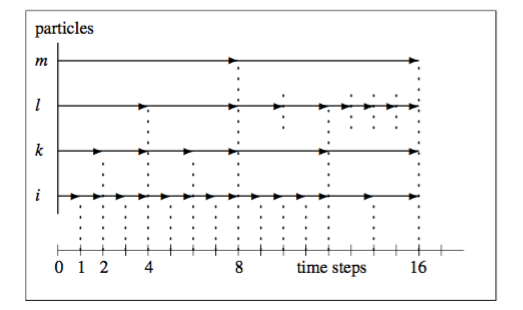
\includegraphics[width=\textwidth]{KhalisiTimeStep}
    \caption{Particles $i$, $k$, $l$, and $m$ have separate time steps. A full force computation is done at each arrow, otherwise, the position and velocity are extrapolated from the values already computed.  These time steps are reevaluated by equation~\ref{eqn:blocksteptime} after a full integration cycle. Subsystems which are evaluated independently are replaced by their center of mass in the block scheme. Figure reproduced from \citet{2017Khalisi}.}
    \label{fig:blockstep}
\end{figure}

The \nbody employs the neighbor scheme of \citet{1973Ahmad} in conjunction with the Hermite integrator and block timestep. This is a further optimization to speed up the calculations, this time by identify particles that are spatially close to each other. Thus, a given particle will actually have two timesteps, a regular timestep and (smaller) irregular timestep. Particles have a neighbor list of size at most $N_{\mathrm{nb}} \ll N_{\mathrm{tot}}$.  These are advanced using a similar predictor-corrector as the Hermite scheme above, computing the full force for neighbor particles and the last regular values for non-neighbors. Membership in the neighbor list is determined by the size of the neighbor sphere and the length of the neighbor list $N_{\mathrm{nb}}$.  The first $N_{\mathrm{nb}}$ particles within a sphere of radius $r_{\mathrm{search}}$ are included.  We found that too small values for $N_{\mathrm{nb}}$ would lead to code crashes and settled on a value of 1024.  We use a search sphere of radius $1 \times 10^{-4} \pc$.

The distinguishing feature of the \texttt{NBODY} family is their use of \citet{1965Kusta} (KS) regularization to generate solutions for binaries, triples, and multiple systems with high levels of accuracy.  This treatment for close encounters adds a good deal of complexity to the implementation, but the scheme essentially works by searching for bodies closer to each other than $r_{\mathrm{min}}$, replacing them in the next integration step by their center of mass, and integrating them separately at a smaller timescale and in a different reference frame. This is useful to avoid numerical truncation errors caused by bodies being too close in the originally reference frame. The KS regularization is extended to multiple systems and adds perturbing bodies using a variant of the \citet{1973Ahmad} neighbor scheme. KS pairs and multiples are terminated if the distance between the bodies exceeds $r_{\mathrm{min}}$ or if the bodies collide, in which case they are merged.  We discuss the merger criteria and method later in this section.

Although \nbody uses MPI parallelization to scale across multiple compute nodes, there are some sequential bottlenecks including KS regularization. Figure~\ref{fig:parallelperf} shows the results of our tests scaling to multiple nodes and compares to the theoretical limit.  We also performed profiling which indicated that the bulk of the time was spent in KS regularization. Because we didn't achieve gains from horizontal scaling, we were not able to take full advantage of the computing power available to us.
\begin{figure}
\centering
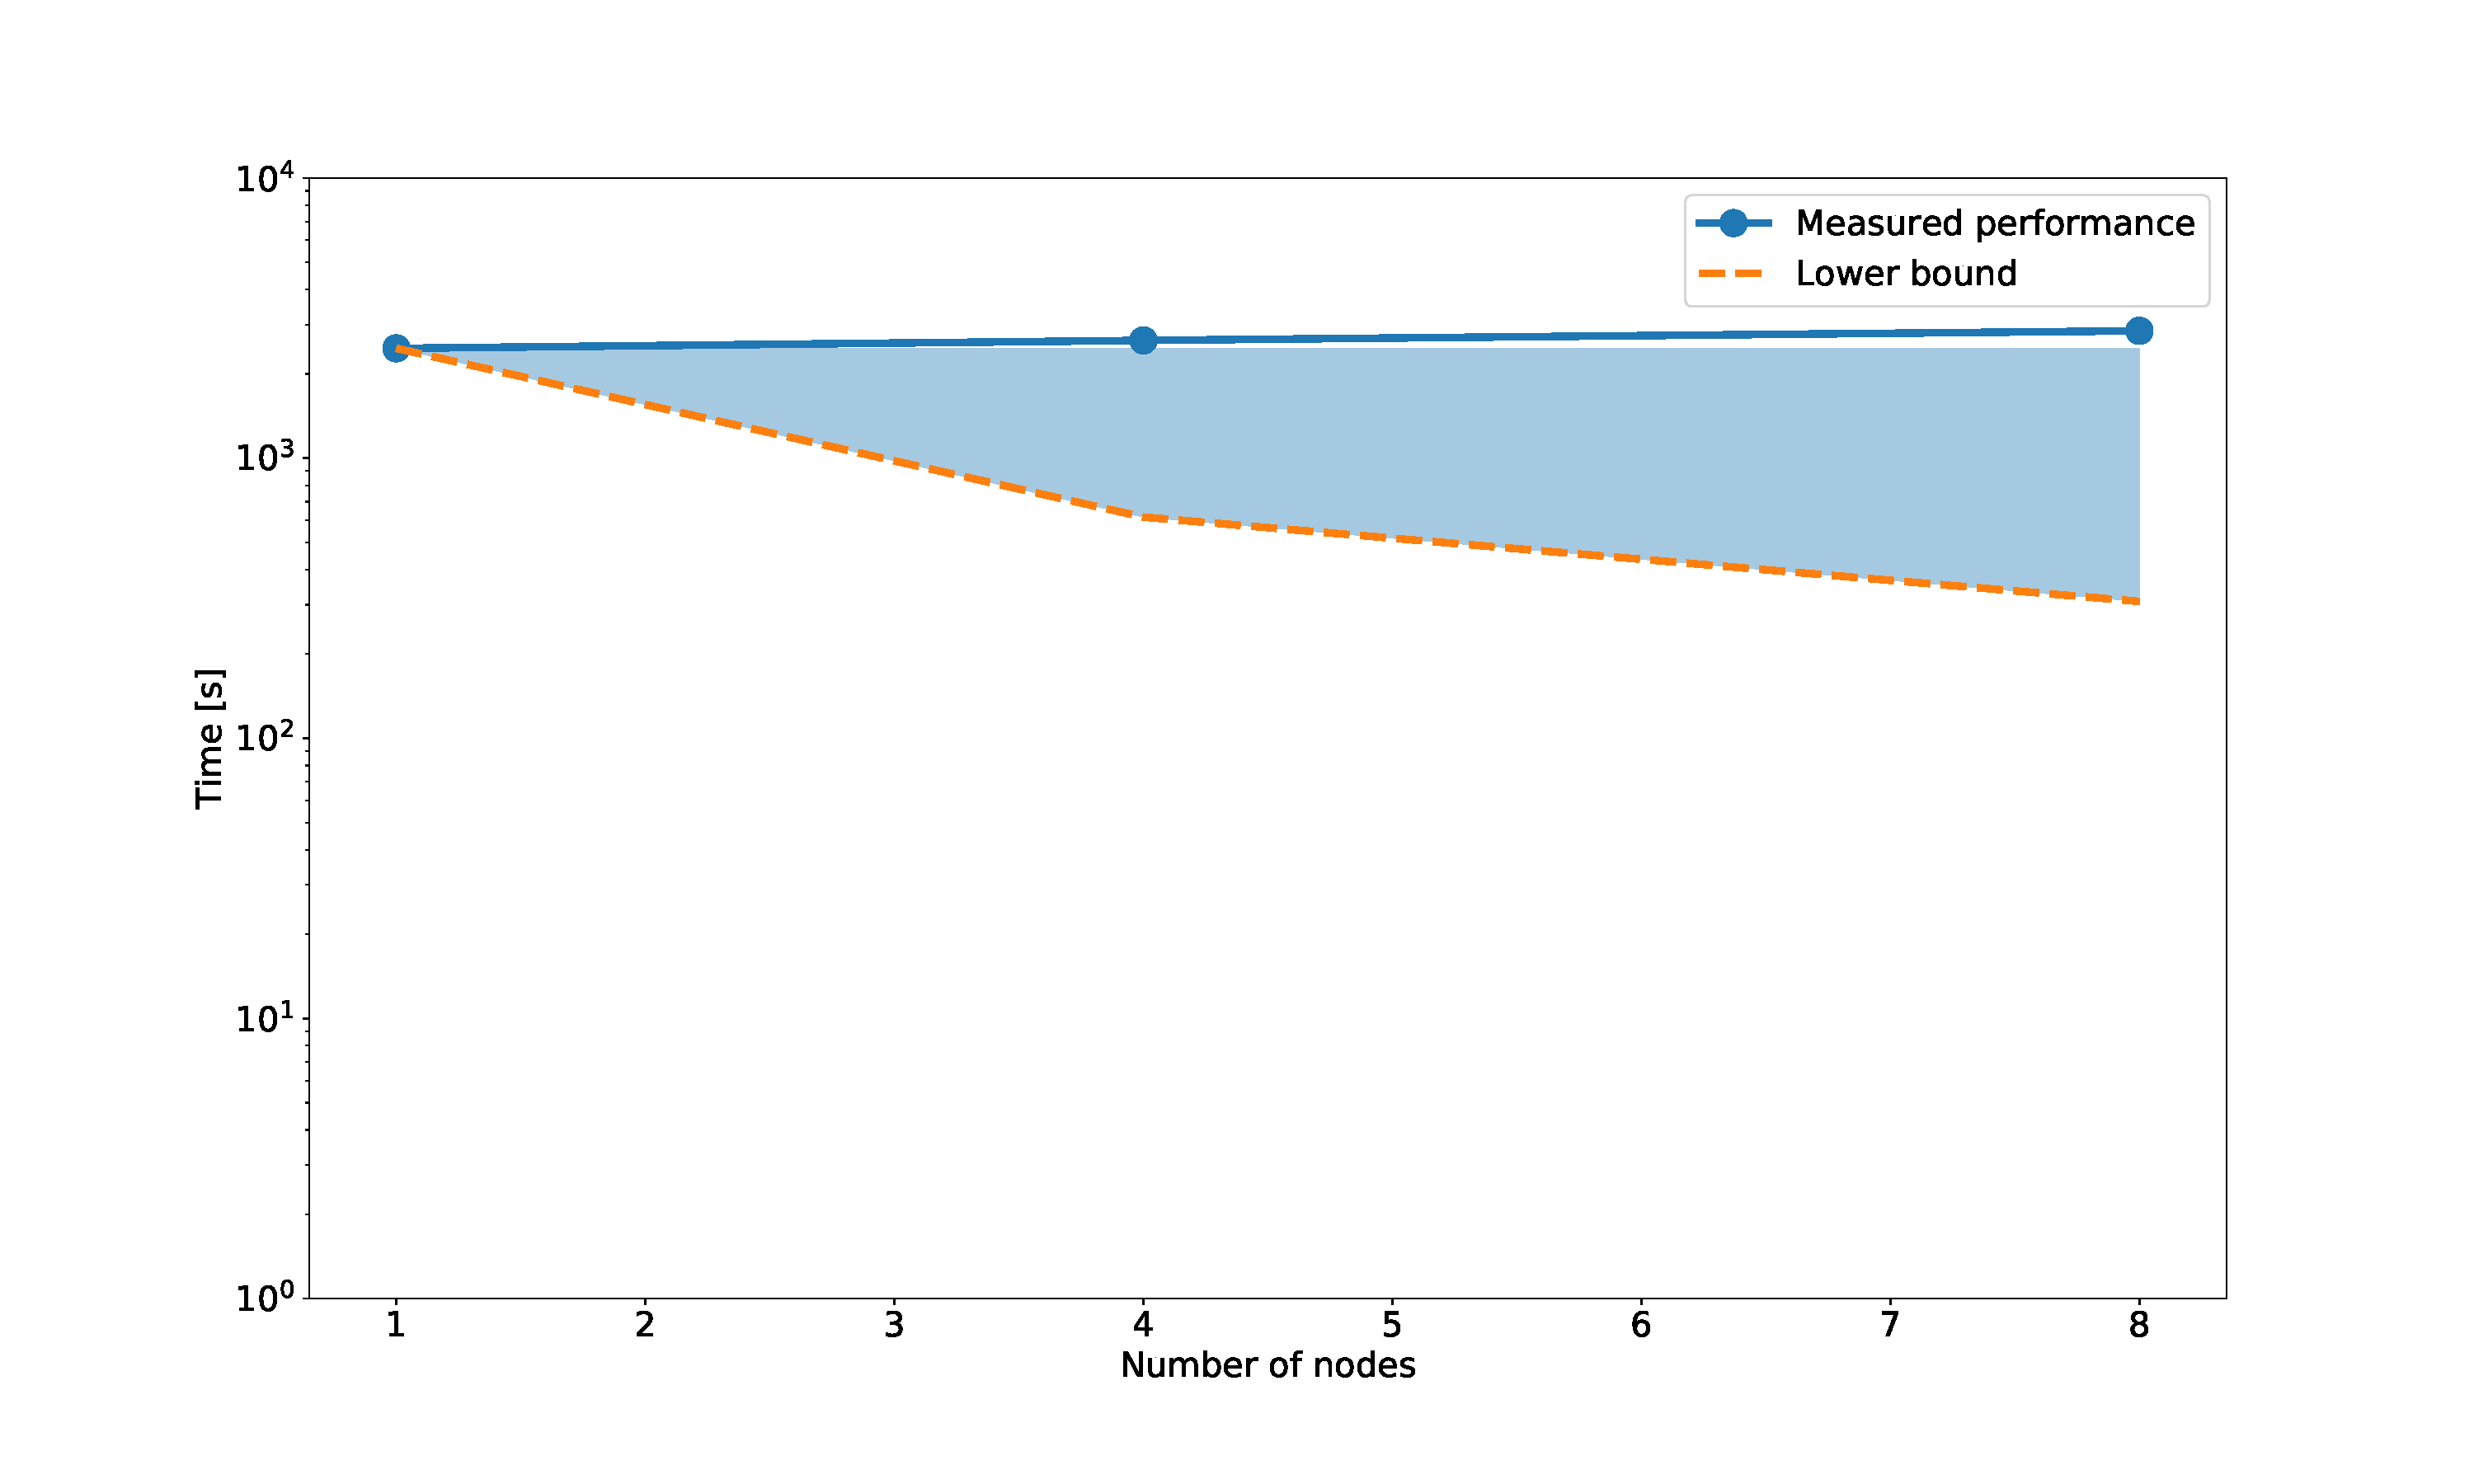
\includegraphics[width=\textwidth]{parallelperformance}
\caption{This figure shows the results of our parallel test runs and compares to the theoretical limit.  The shaded region indicates a range of speedups that we might expect depending on the fraction of parallelizable work following Amdahl's law.  That actual performance was even worse is a result of communication overhead. For all of our parallelization test runs we used identical clusters of 4000 bodies with total mass of 13k $\Msun$ and following a \citet{1966King} profile with concentration 2 and half-mass radius $0.5 \pc$.  Each cluster was evolved to 3 Myr.}
\label{fig:parallelperf}
\end{figure}

We performed our simulations on the \texttt{Tiger2} GPU cluster at Princeton University. Most experiments were performed on one compute node which each use four NVIDIA Tesla P100 GPUs and 2.4 GHz Broadwell processors parallelized with OpenMP.

\section{Initial and Boundary Conditions}
We generate our initial conditions using the \texttt{McLuster} software of \citet{2011Kupper}. For the initial distribution of positions and velocities, we use a \citet{1966King} profile, varying half-mass radius and concentration.  We use the initial mass function of \citet{2001Kroupa} which degenerates to a Saltpeter IMF above $0.5 \Msun$.  For our simulations with cluster mass $2 \times 10^5 \Msun$, we use a mass range of $1$ to $100 \Msun$.  For cluster mass $6 \times 10^5 \Msun$, we increase the lower bound to $3.3 \Msun$.  For cluster mass $2 \times 10^6 \Msun$, we use a lower bound of $13 \Msun$ and an upper bound of $120 \Msun$.  We do not apply an external tidal field, initialize primordial binaries, or apply primordial mass segregation. Figure~\ref{fig:icpanel} shows the initial density profiles for each run.

We use an open boundary condition so particles that do escape do not return to the simulation. Our escape condition is a distance from center of greater than twice the tidal radius. Both of these conditions remain uniform over all of our simulations.

\begin{figure}
\centering
\makebox[\textwidth]{\includegraphics[width=\paperwidth]{icpanel}}
\caption{Initial density profile for each run.  We computed the density profiles by binning stars in groups of 32 and taking the average mass over the spherical volume they occupy, so the noise in the density curves is because without primordial mass segregation more massive stars can have a strong influence on the total mass within their bin.}
\label{fig:icpanel}
\end{figure}

\section{Merger Scheme}
The default merger criteria in \nbody follows that of \citet{1992Kochanek}.  For a two-body system with pericenter $R_p$, the bodies are merged if

\begin{equation}
 \frac{R_{p}}{R_{1}} \leq 1.3 \times (\frac{M_T}{2M_1})^{1/3}.
 \label{eqn:kochanekcriteria}
\end{equation}

This merger scheme is conservative.  In the case of a central mass with $m = 200 \Msun$ (a typical case after a couple of mergers) and an additional mass with $m = 1 \Msun$, and using $r_{\mathrm{central}} = (\frac{m}{\Msun})^{0.55}$, we would not merge the two stars unless they had a pericenter distance smaller than $20$ stellar radii, or a deviation of only about $3\%$ from the radius of the central mass.

In an effort to increase the speed of our simulations by spending less time in KS regularization for insignificant bodies, we experimented with short-circuiting this merger scheme for pairs meeting certain conditions.  We experimented with merging binaries where one member was $5$ or $10$ times larger than the other, provided the pericenter distance was smaller than $10 r_\mathrm{large}$ (in the more conservative trial) and $100 r_\mathrm{large}$ in the more liberal one.  We avoided merging with the central mass, but did want to reduce the number of KS pairs for peripheral bodies. We found that the overall runtime was not affected significantly by this change to the merger scheme. Simulation results appeared robust to the factor $10$ difference, but were affected by the factor $100$ difference.  We tested changes to our merger scheme at approximately the transition between collisional and non-collisional clusters: a mass of $2 \times 10^5 \Msun$, a concentration of $2$, and a half-mass radius of $2.9 \pc$.

\section{Verification}
\citet{2009Anders, 2012Anders} perform comparisons between \texttt{NBody4} of \citet{1999Aarseth} and \texttt{Starlab} environment.  In order to verify our installation of \nbody we repeated the tests from \citet{2009Anders}.  We used \texttt{McLuster} to generate similar initial conditions to the ones used in their test. Our verification clusters consist of 1024 $1 \Msun$ stars, distributed in a Plummer profile with initial half-mass radius $0.5 \pc$.  We performed test runs with and without stellar evolution mass loss, as \nbody requires stellar evolution mass loss to perform mergers.

The trends of our verification runs generally agreed with those in \citet{2009Anders}.  The authors left some uncertainty about the exact parameters used for their runs, and they also sampled many runs to obtain an average. Figures~\ref{fig:verifications1} and ~\ref{fig:verifications2} compare the two.

\begin{figure}%
    \centering
     \subfloat[Half-mass radius vs. time reproduced from \citet{2009Anders}.]{{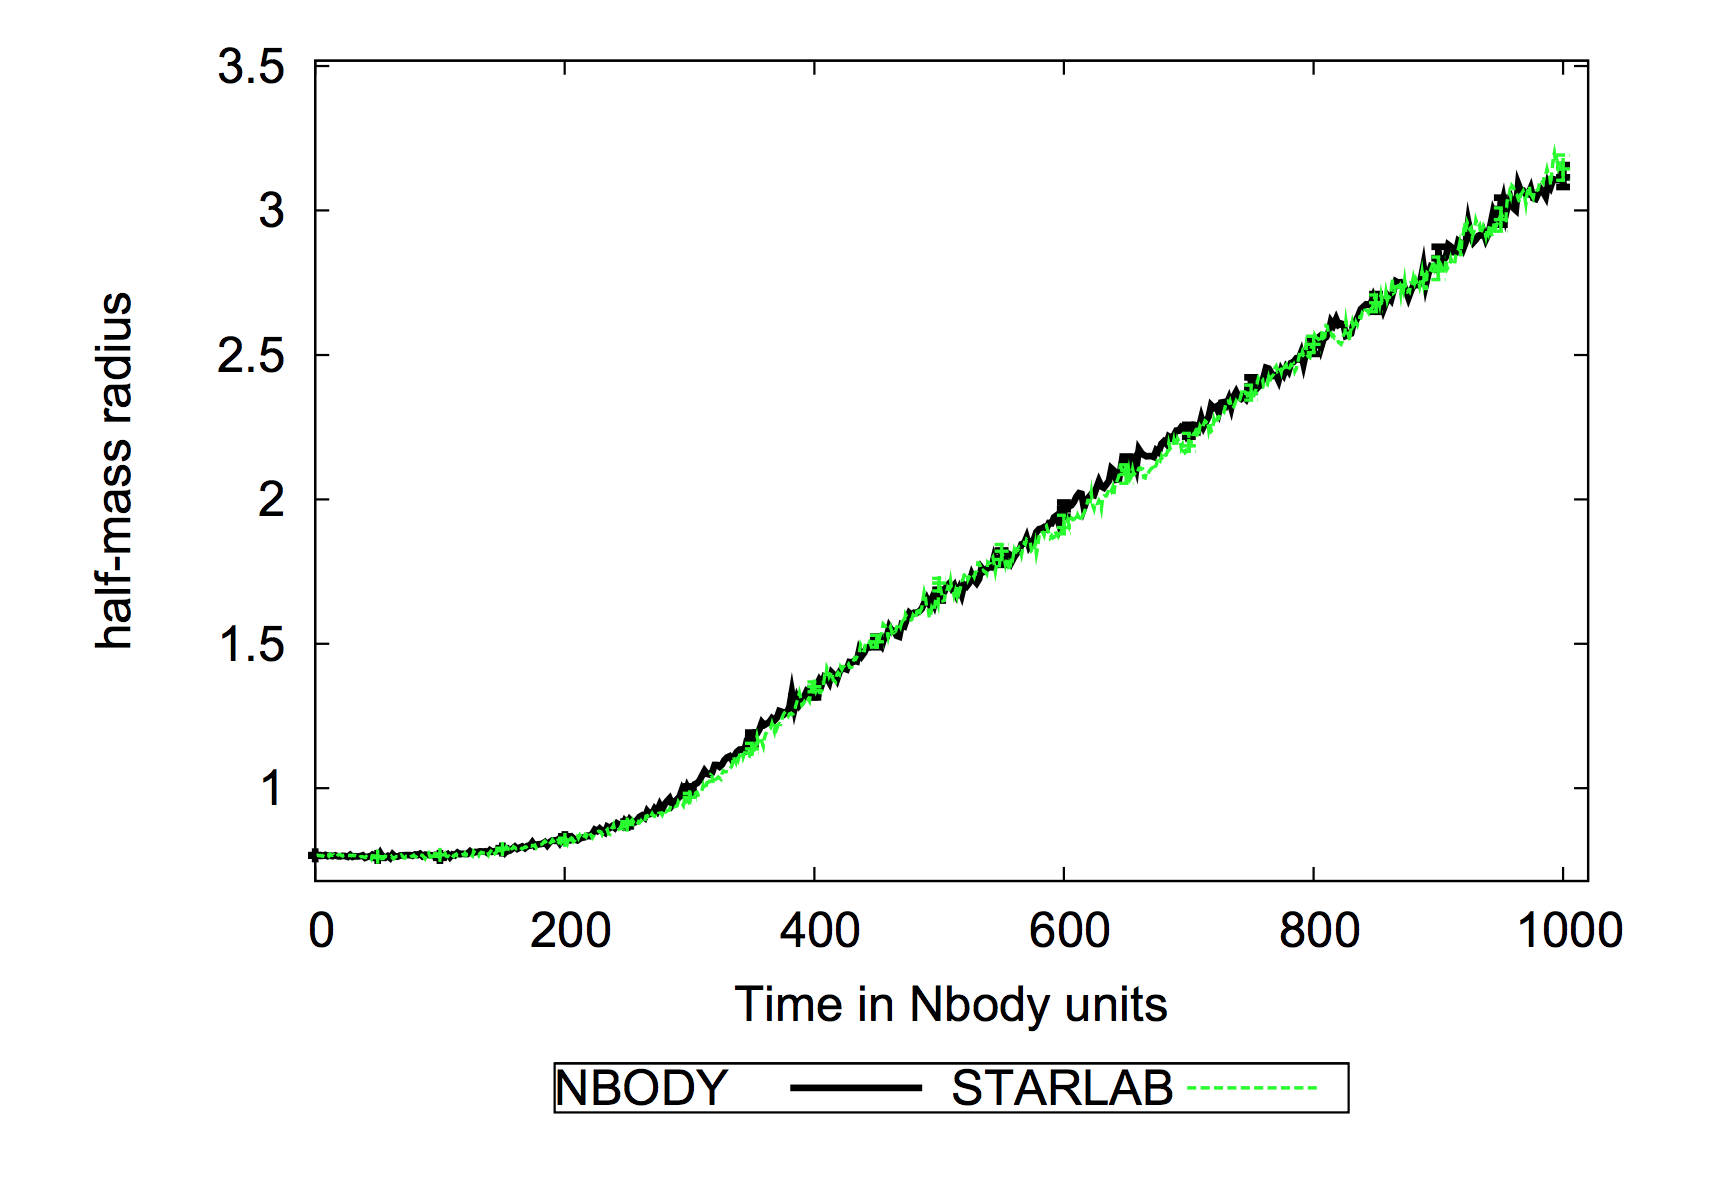
\includegraphics[width = 7cm]{AndersHalfRadius}}}%
    \qquad   
    \subfloat[Core radius vs. time reproduced from \citet{2009Anders}.]{{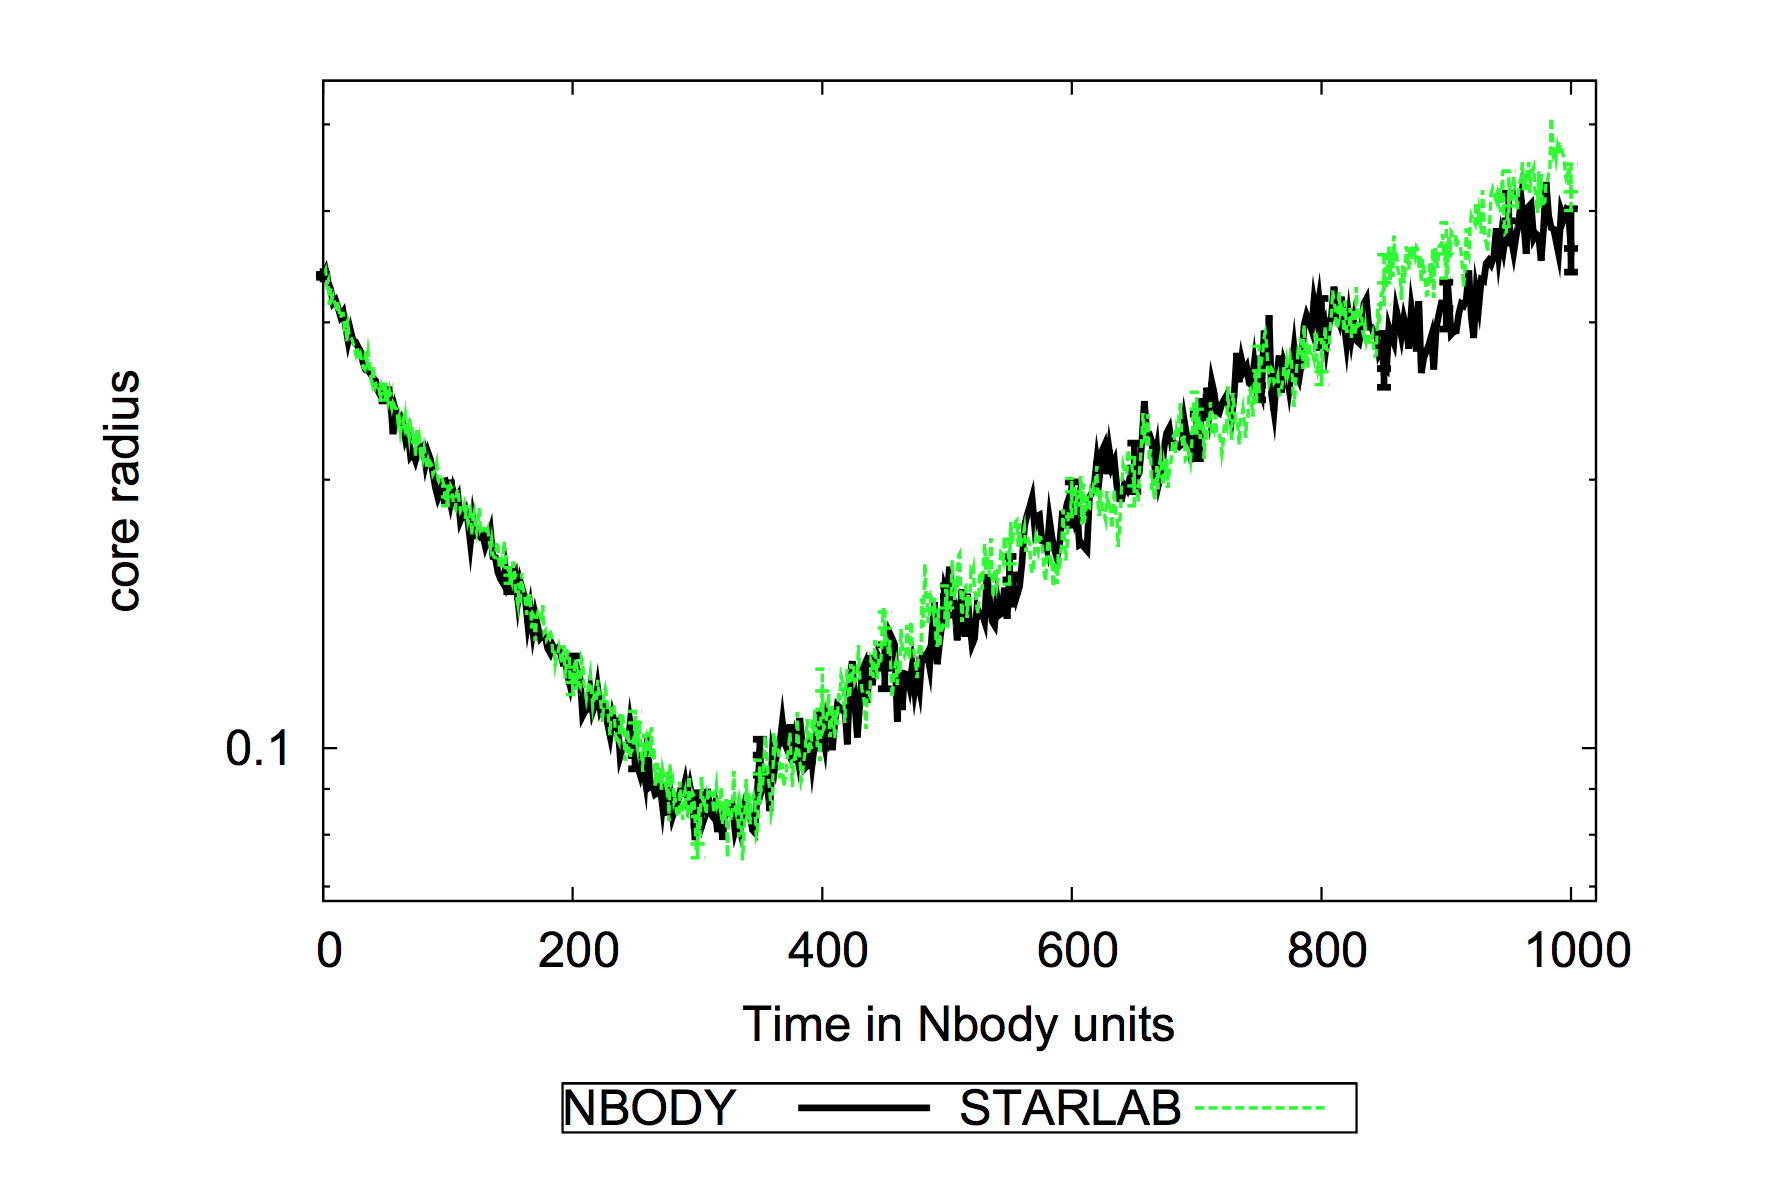
\includegraphics[width = 7cm]{AndersCoreRadius}}}%
    \qquad
    \subfloat[Half-mass radius vs. time from our verification run.]{{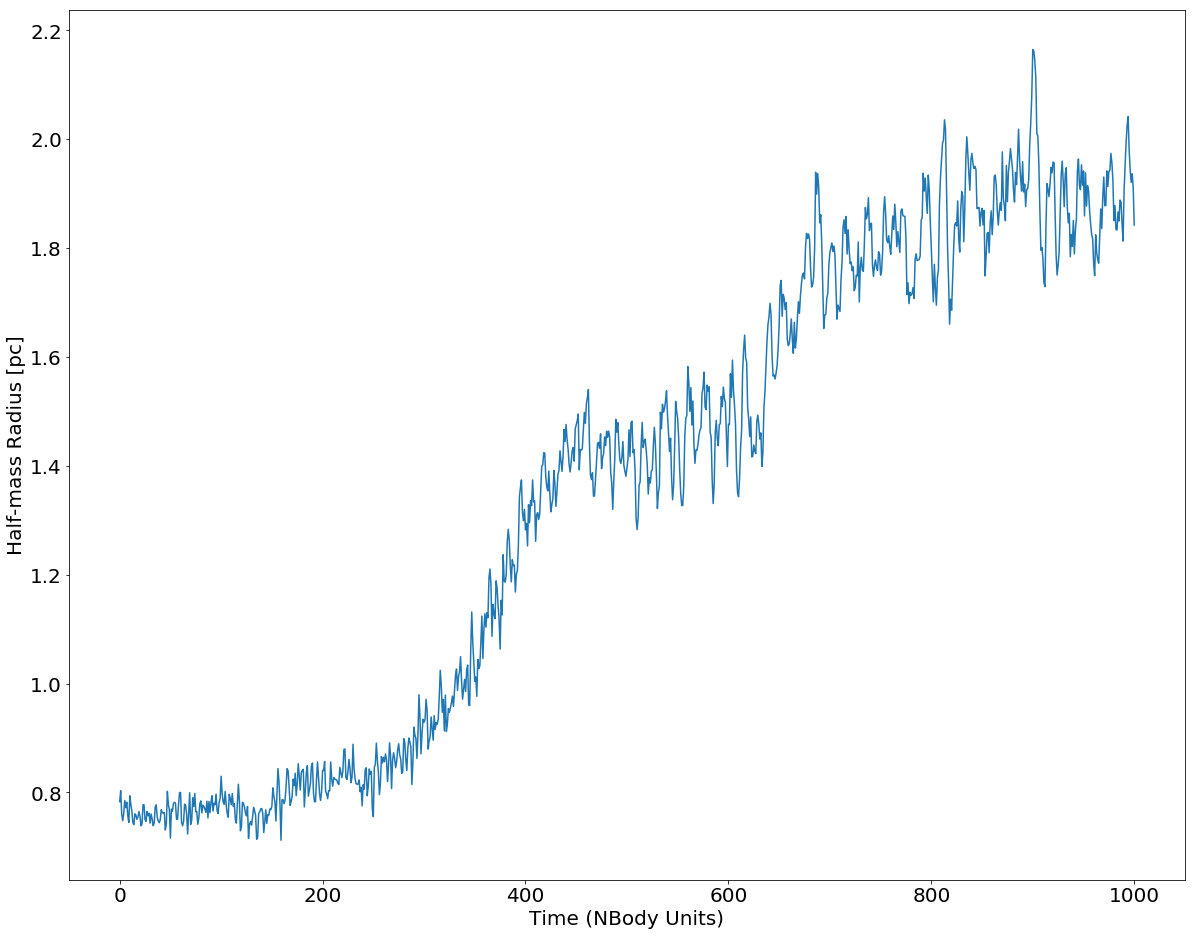
\includegraphics[width = 7cm]{VerifyHalfRadius}}}%
    \qquad
    \subfloat[Core radius vs. time from our verification run.]{{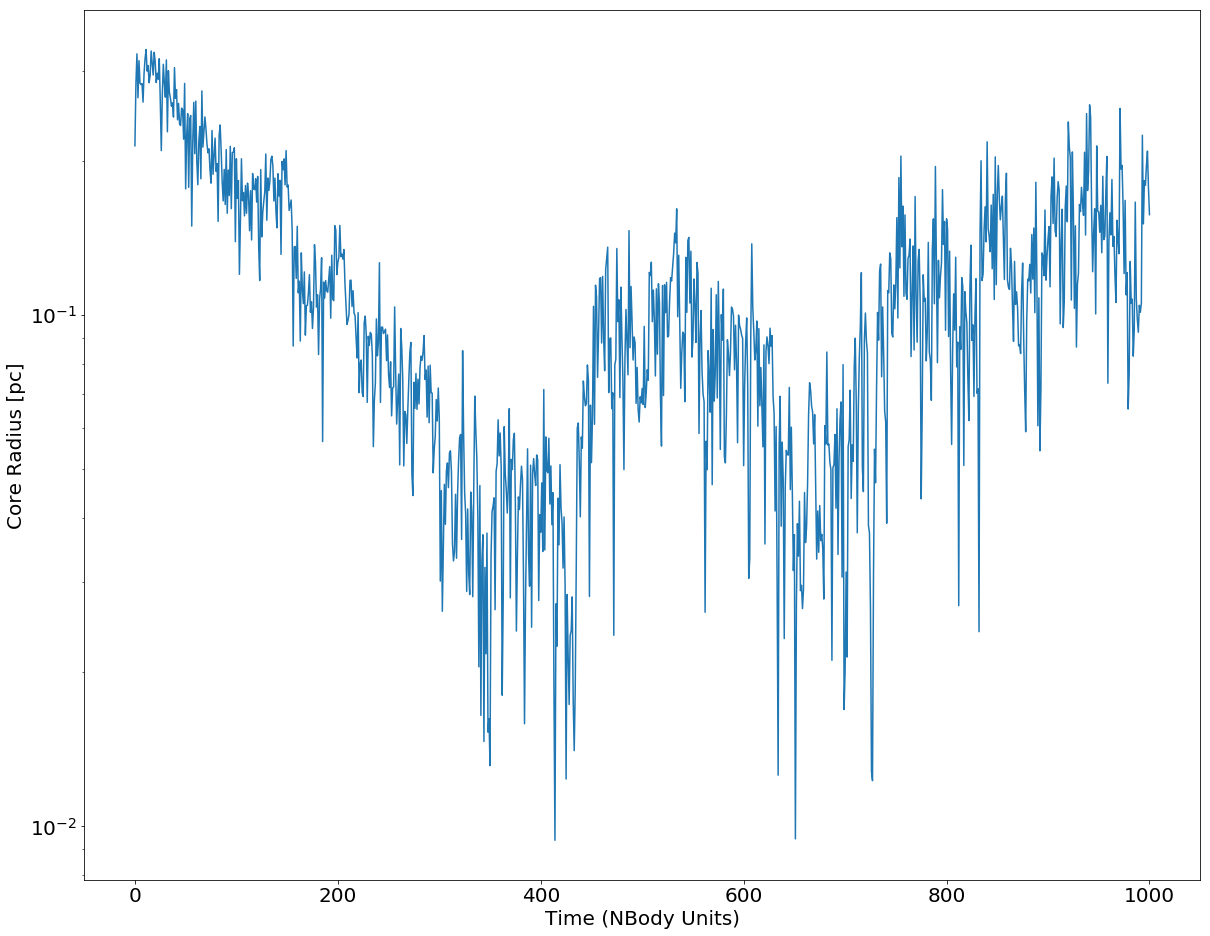
\includegraphics[width = 7cm]{VerifyCoreRadius}}}%
    \caption{Our verification run shows generally good agreement with those of \citet{2009Anders}.  The half mass radius doesn't start to expand significantly until $200$ time steps in both sets, and then follows a general upwards trend.  Our core radius shows a similar peak-trough distance of oscillation and a return close to the starting point by the end of the run.
    Our result appears to oscillate more because we show a single run instead of an entire sample. }
    \label{fig:verifications1}
\end{figure}

\begin{figure}%
    \centering
     \subfloat[Kinetic energy vs. time reproduced from \citet{2009Anders}.]{{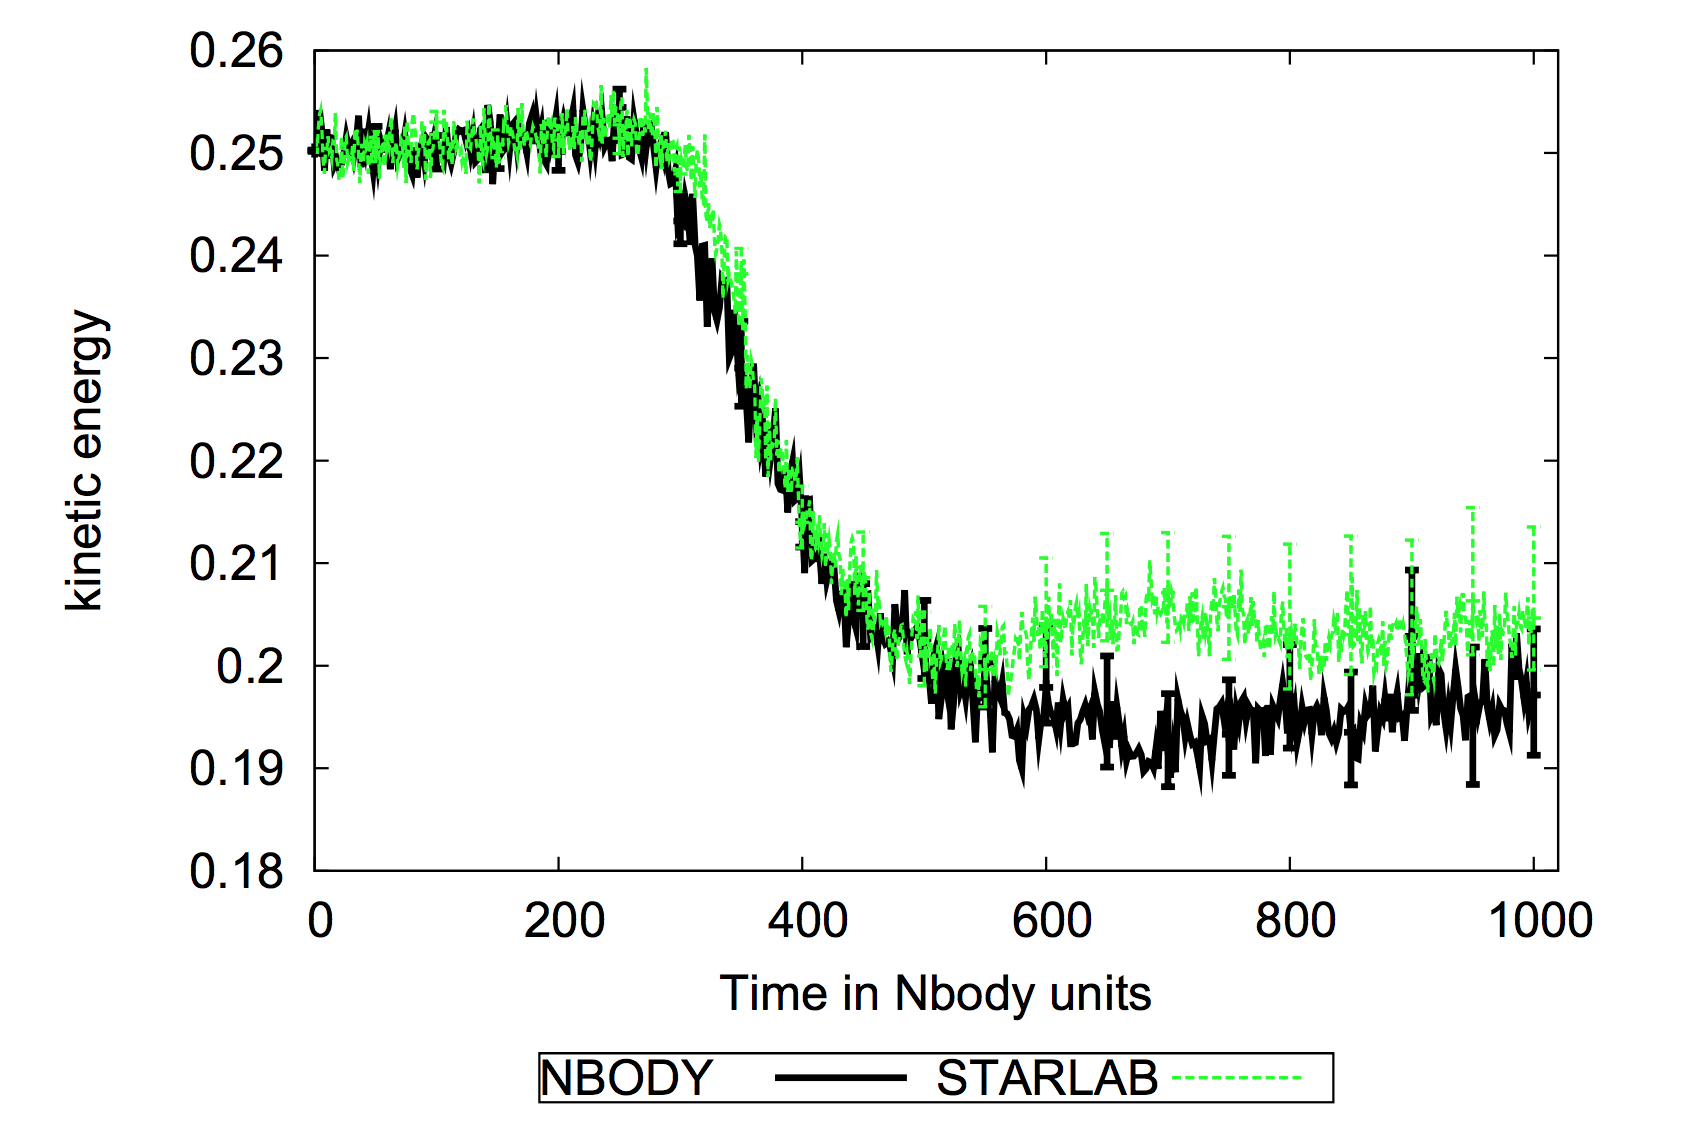
\includegraphics[width = 7cm]{AndersKinetic}}}%
    \qquad   
    \subfloat[Potential energy vs. time reproduced from \citet{2009Anders}.]{{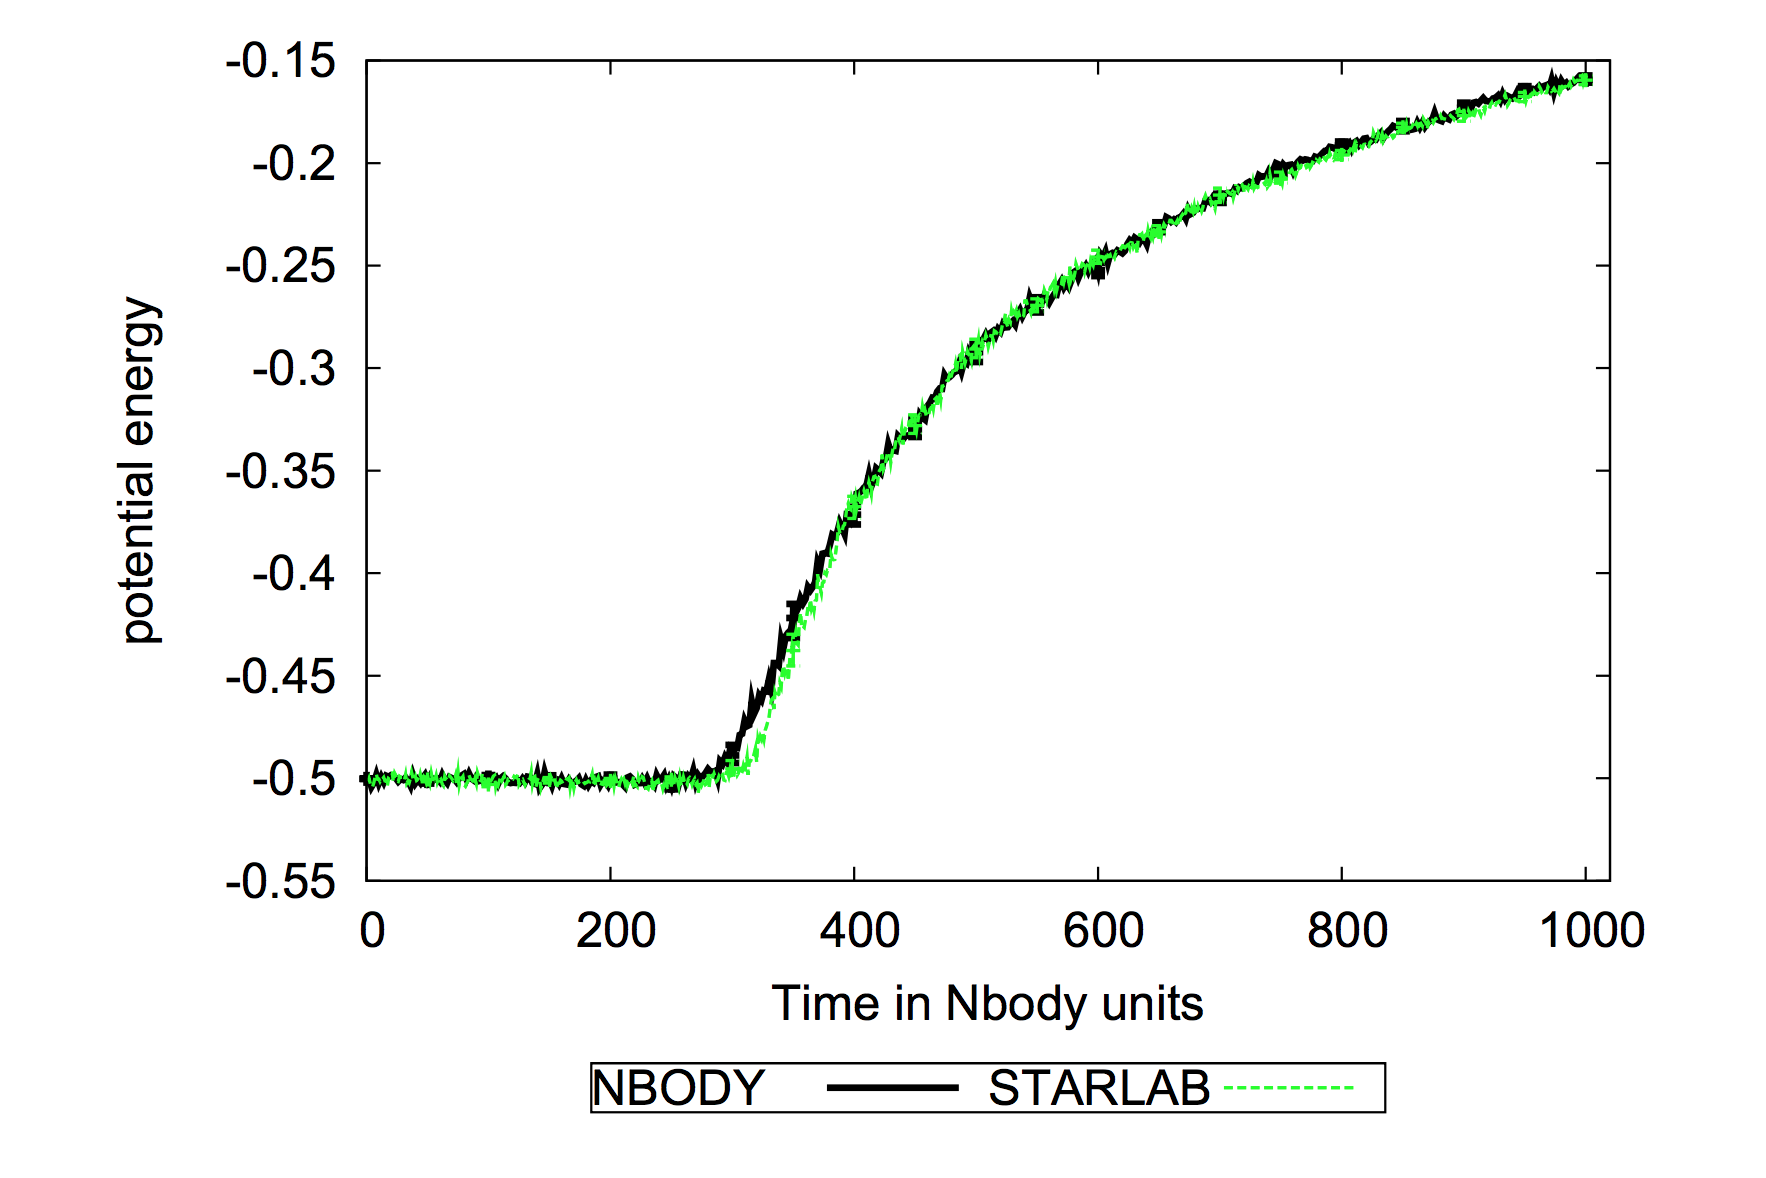
\includegraphics[width = 7cm]{AndersPotential}}}%
    \qquad
    \subfloat[Kinetic energy vs. time from our verification run.]{{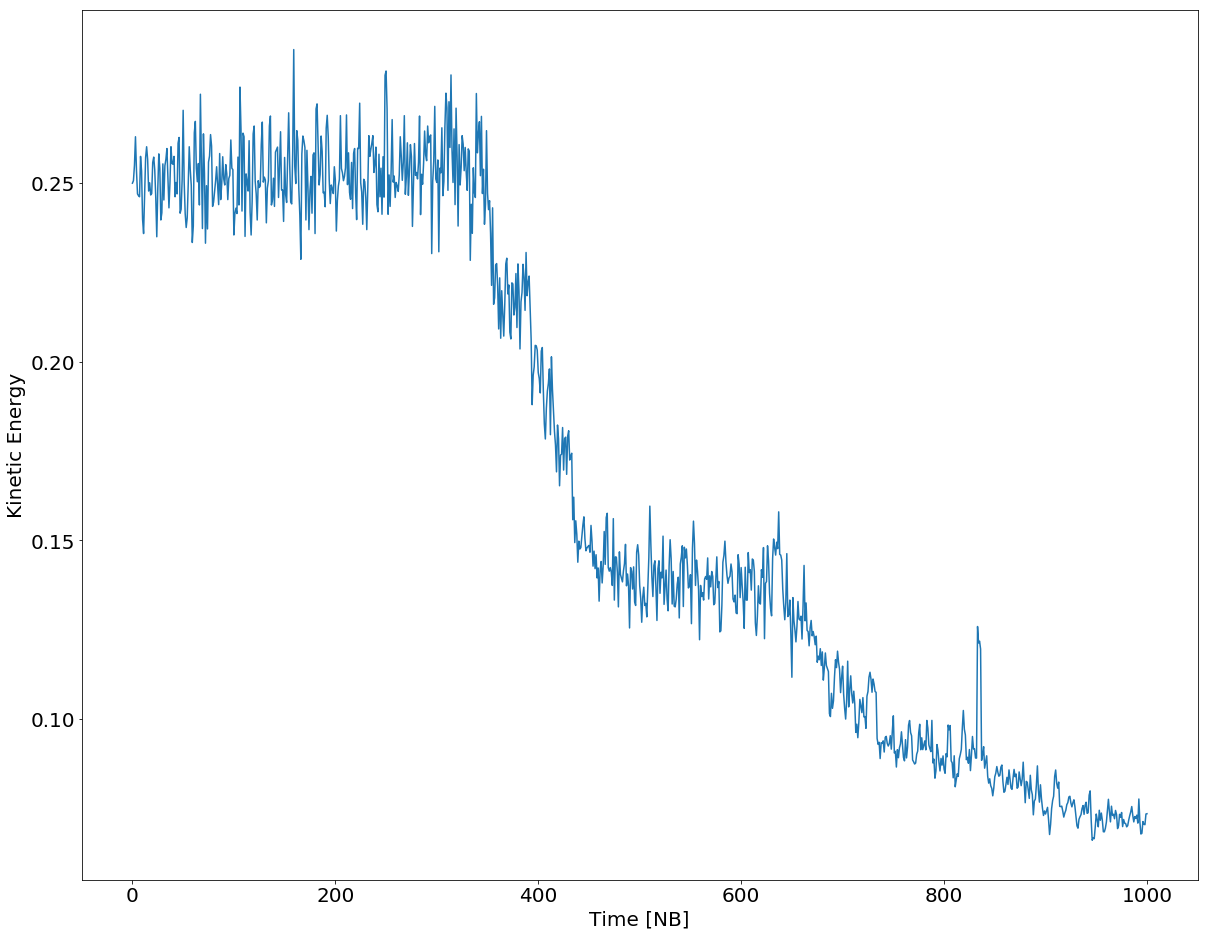
\includegraphics[width = 7cm]{VerifyKinetic}}}%
    \qquad
    \subfloat[Potential energy vs. time from our verification run.]{{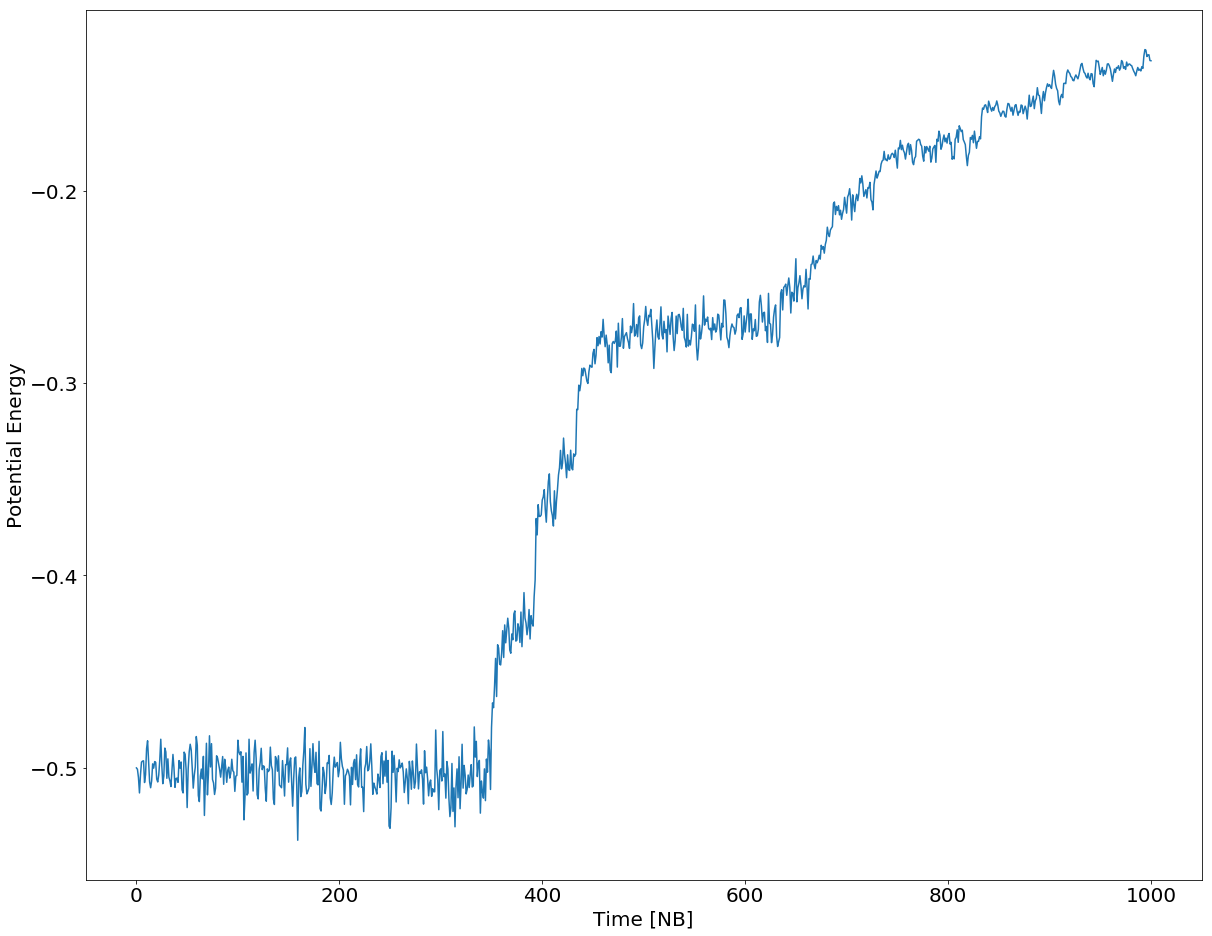
\includegraphics[width = 7cm]{VerifyPotential}}}%
    \caption{We see the same general trend with kinetic and potential energy from our verification run, although the kinetic energy from our run seems to end up lower than that of \citet{2009Anders}.  This is where there is also the greatest divergence between \texttt{NBODY4} and \texttt{Starlab}, so it's possible that changes in between \texttt{NBODY4} and \nbody account for this difference.}
    \label{fig:verifications2}
\end{figure}


\section{Additional Modifications}
We had significant difficulty running more collisional clusters to completion.  We found that clusters with many collisions stretched the limits of default \nbody parameters.  Among other issues, we encountered a persistent problem where runs would stop progressing during a KS regularization.  We settled on a two-part workaround for this problem: first by reducing the KS step size which seemed to forestall these failures at the cost of some additional compute time and second by simply restarting runs once they stopped progressing. 

We were unable to get \nbody's internal restart module to function in our environment, so our restart method required building a tool to parse the checkpoint data and create initial conditions for a fresh simulation.  The raw checkpoint data does not perfectly reflect the state of the system because it contains duplicate bodies when binaries, triples, quads, and chains are involved. We implemented an additional heuristic in our restart code to remove spurious binaries and other multiples, leaving only the constituent bodies in the new initial conditions.

\nbody's default configuration does not always seem to handle collisional clusters well. This led to other failure modes for our simulations which we tried to correct. In dense clusters we found that the neighbor lists would rapidly become full leading to code crashes.  Here we tried reducing the size of neighbor search spheres per the suggestion of \citet[][personal communication]{2017Wang}, which did not resolve the issue, so we instead doubled the size of the neighbor lists which was enough to alleviate the issue. Another failure mode which we have not yet been able to find a solution to occurs after restarts during GPU force initialization. It appears some initial conditions cause GPU out-of-memory errors which cause \nbody to crash. The resolution we have adopted for that failure mode is to binary search snapshots until finding one that proceeds and begin the run at that point.  We then have to invalidate data after the selected snapshot.

\chapter{Results} \label{ch:Results}

\begin{sidewaysfigure}[ht]
    \centering
    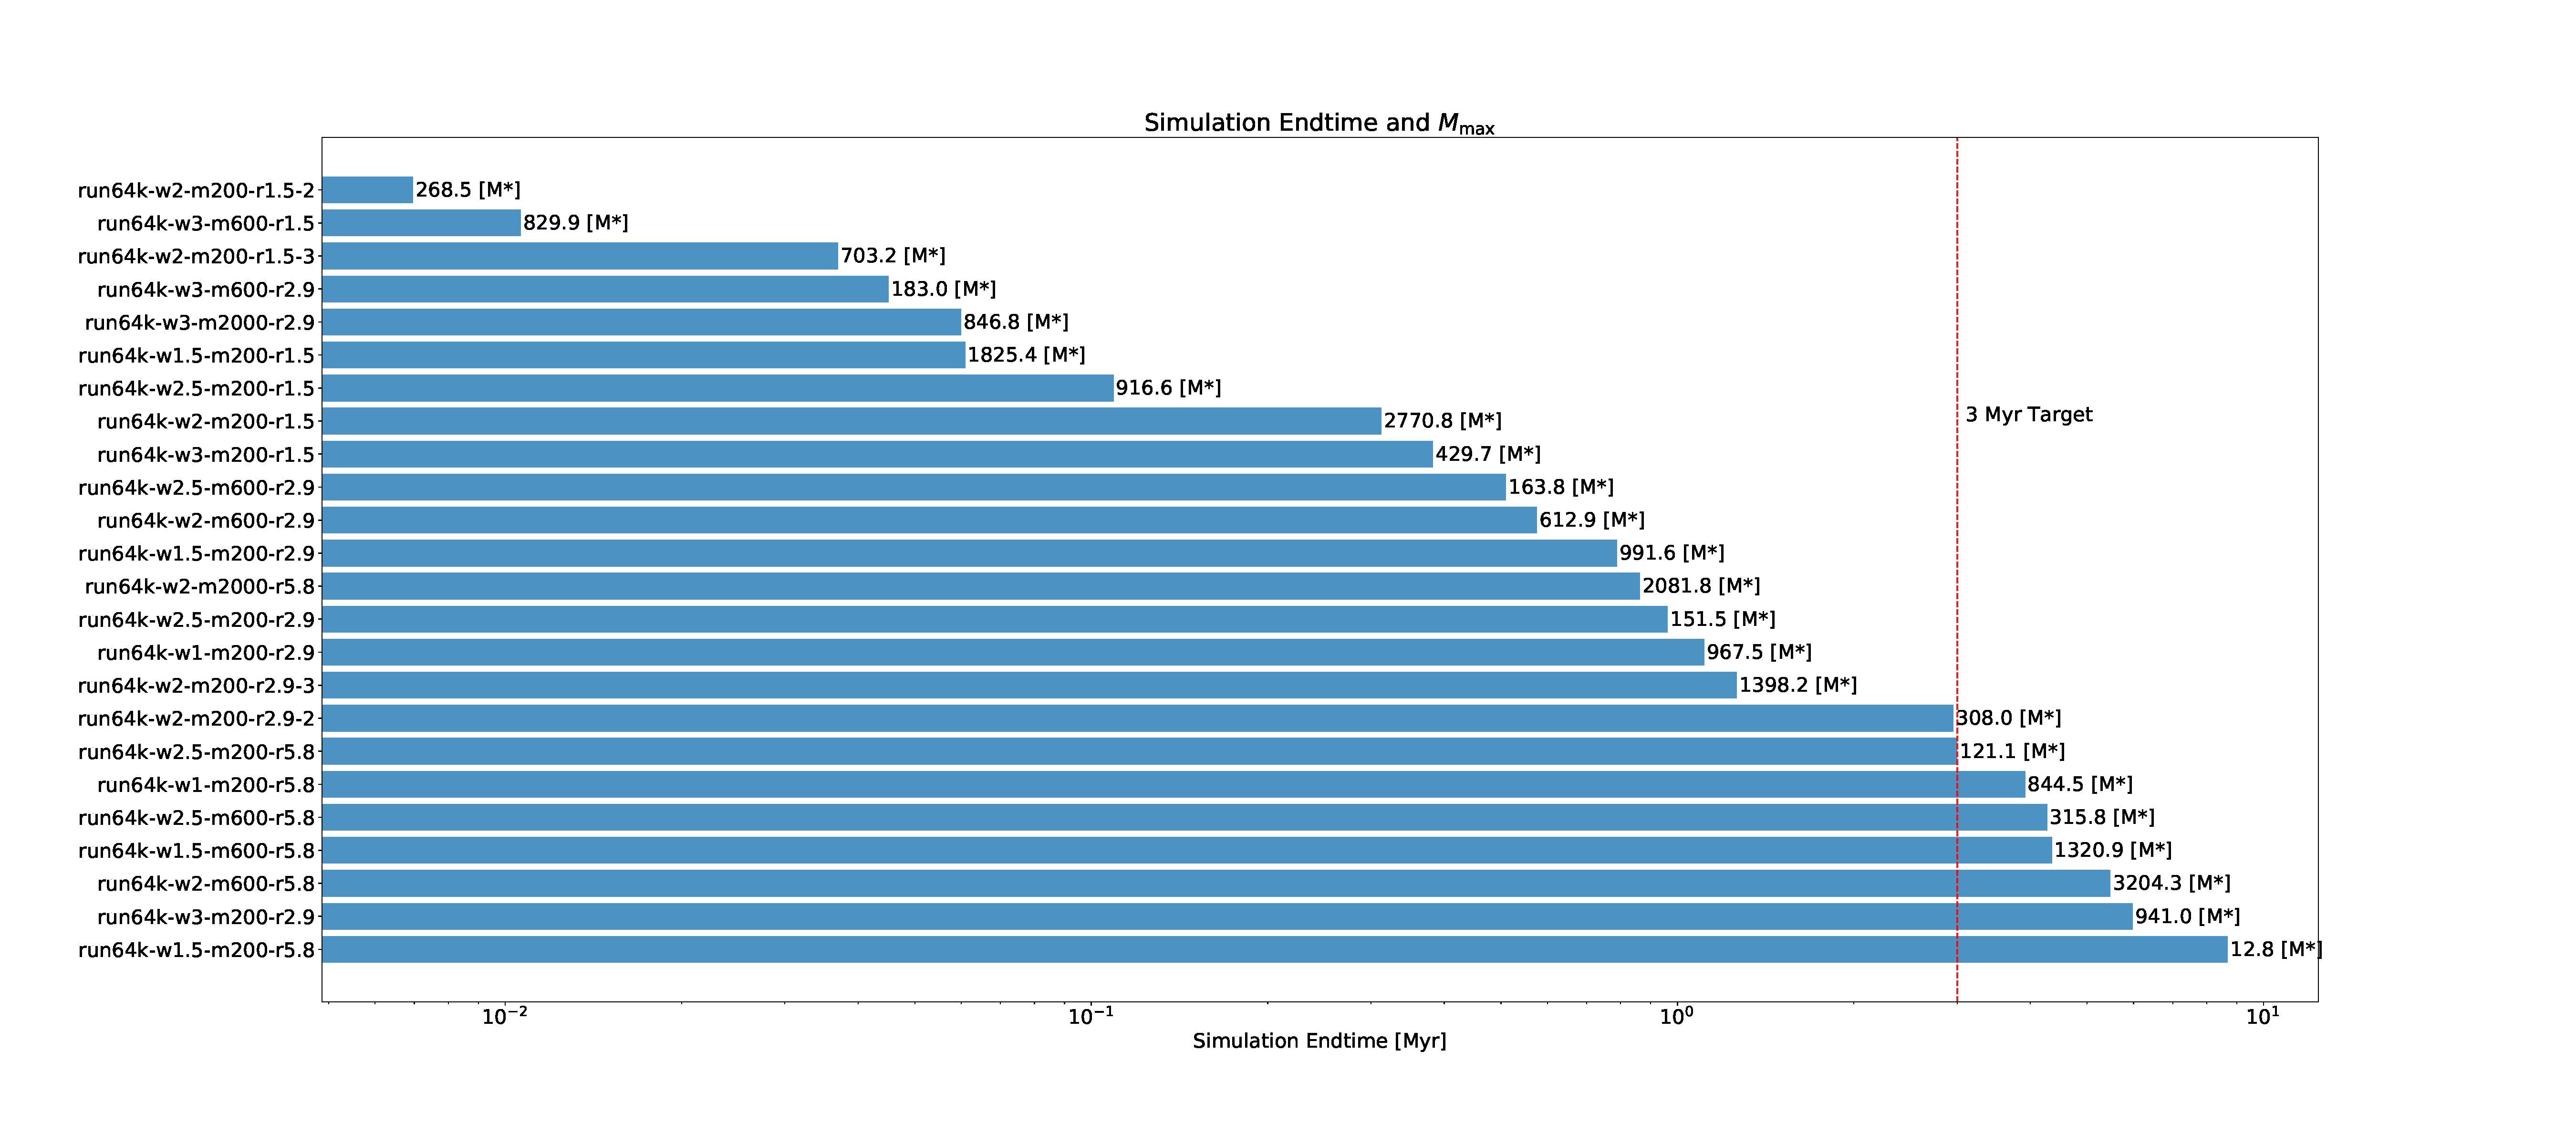
\includegraphics{JobProgress}
    \caption{Not all jobs ran to completion. Integrator performance seemed to struggle most when the central star had many neighbors.  Clusters with more significant mass loss tended to progress more quickly, as many of the stars were ejected leading to quadratic gains.  Some runs were halted because of as-yet undiagnosed code errors in \nbody.}
    \label{fig:JobProgress}
\end{sidewaysfigure}

\begin{figure}
    \centering
    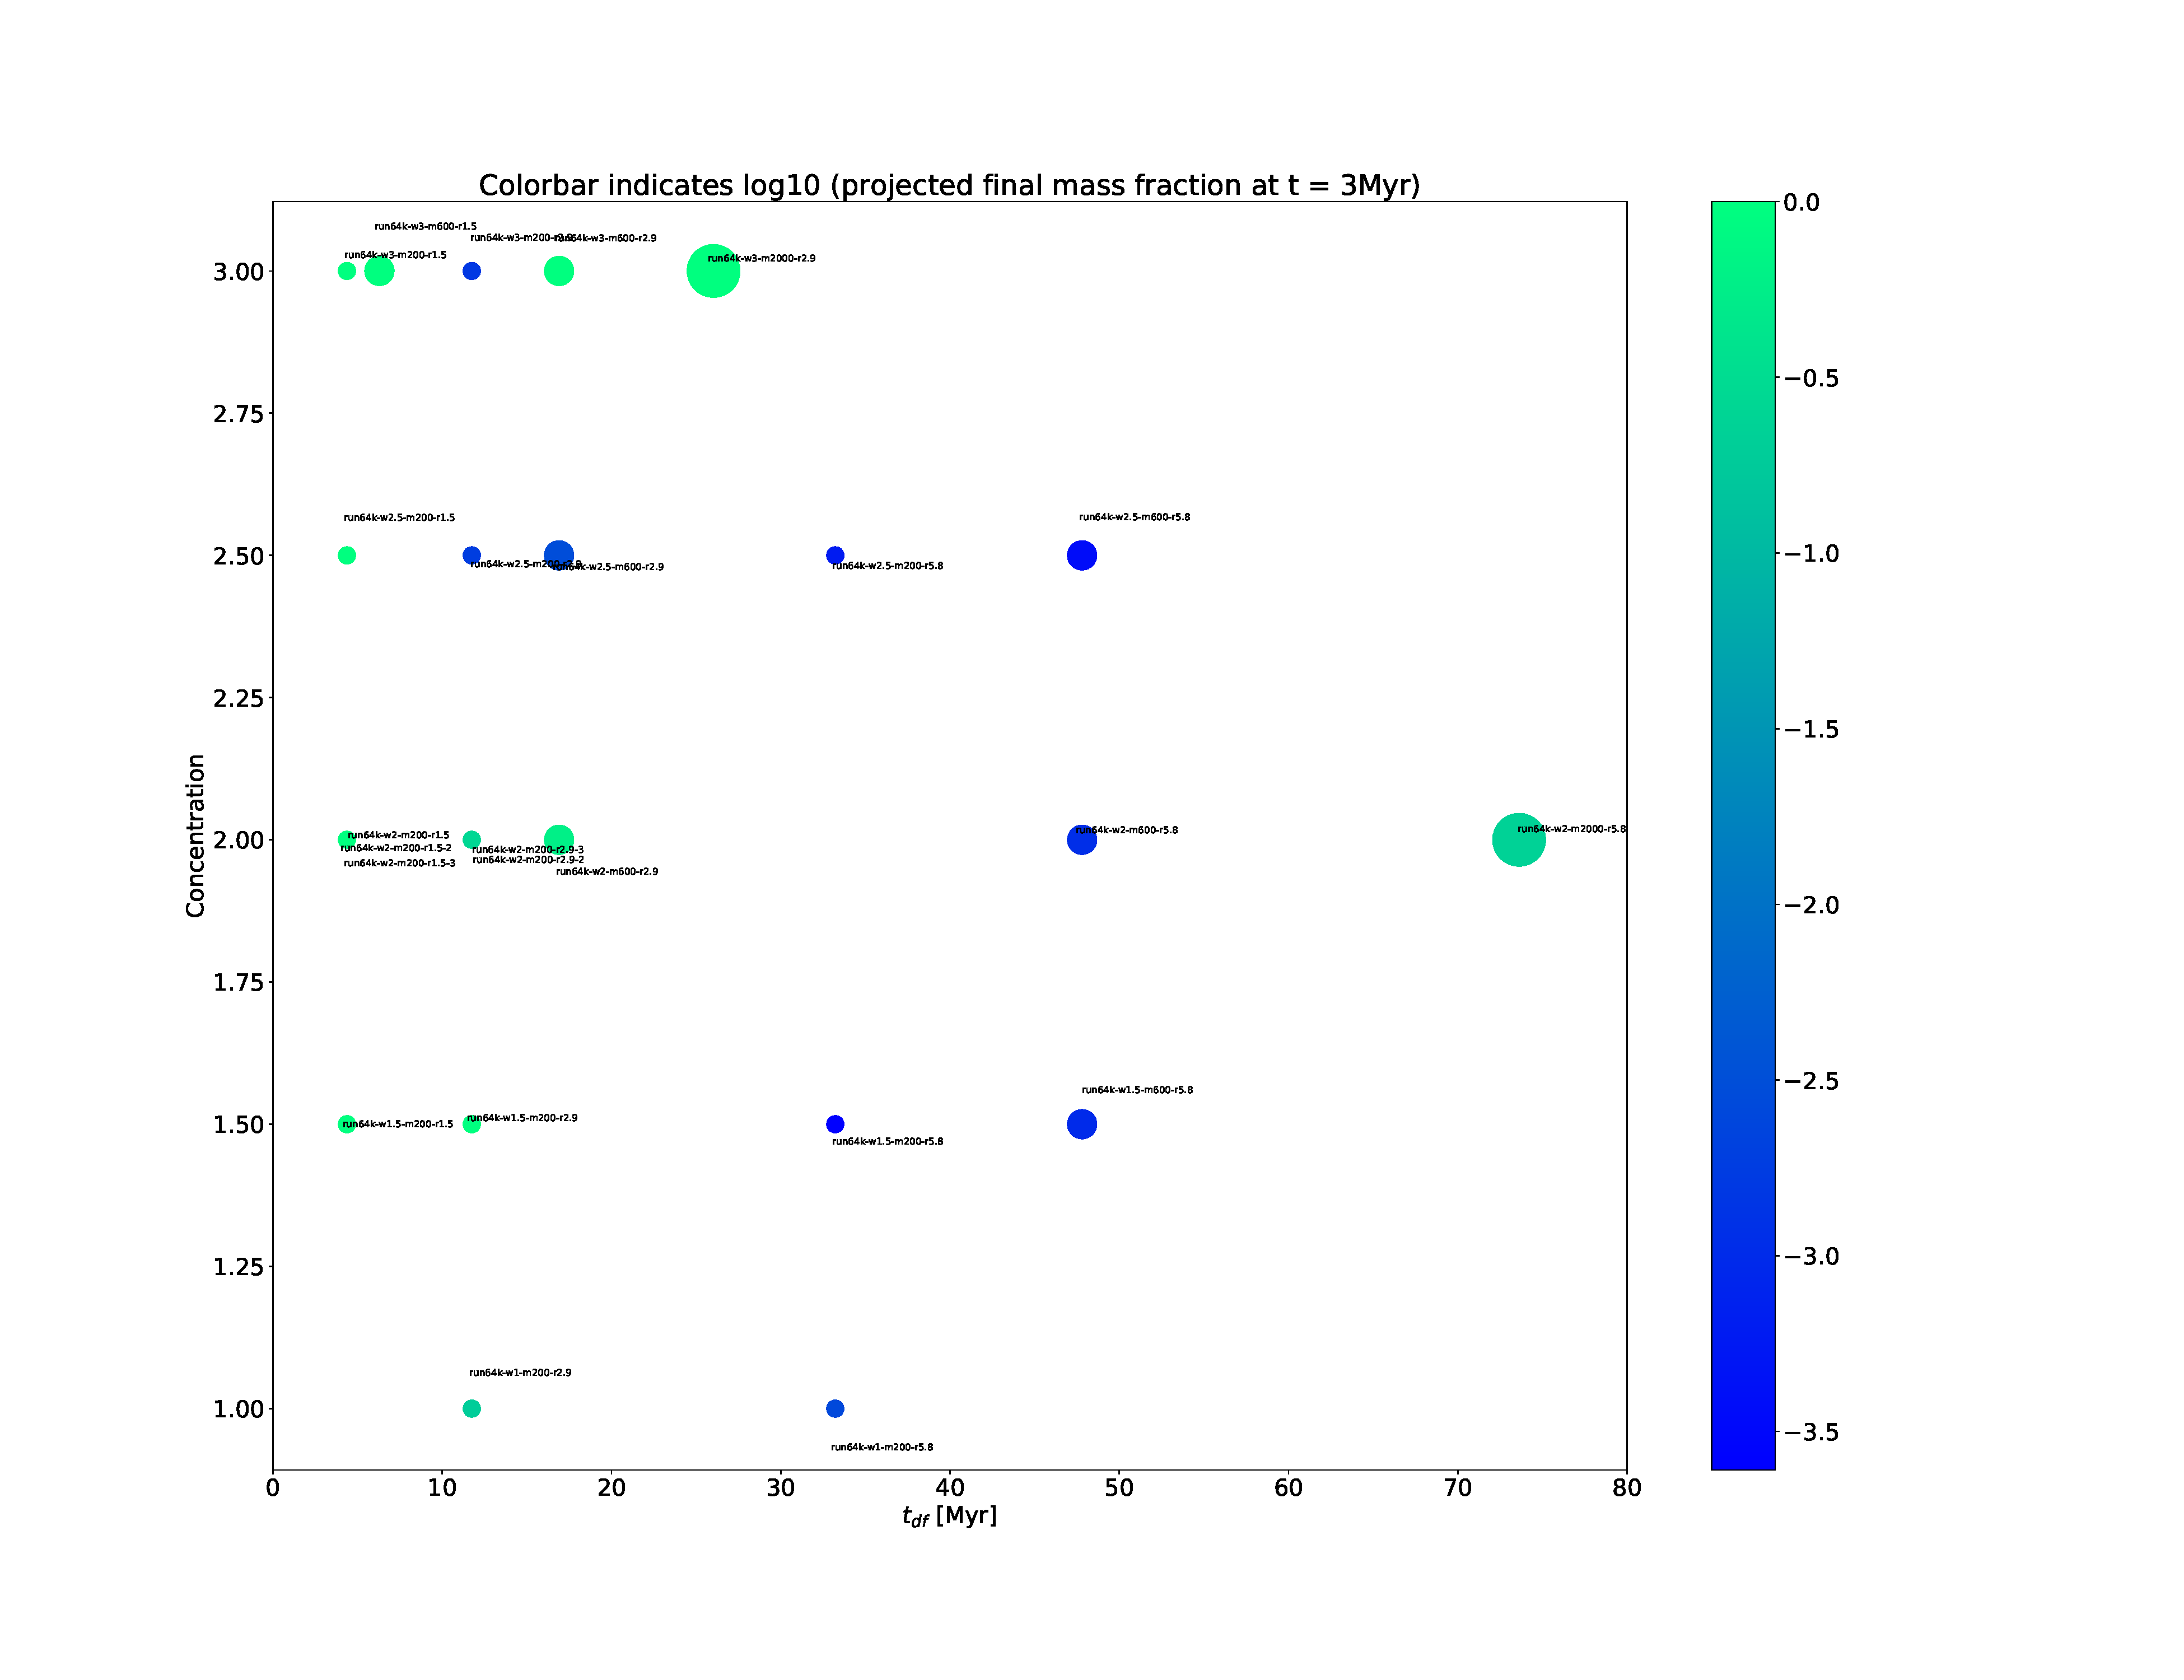
\includegraphics[width=1.3\textwidth]{kplot}
    \caption{The x-axis is the dynamical friction time corresponding to each cluster from equation~\ref{eqn:tdf}.  The y-axis is the concentration parameter.  The clusters are colored by the log of $\mathrm{min}(M_{\mathrm{max, proj}}/M_{\mathrm{total}}, 1)$, where $M_{\mathrm{max, proj}} = M_{\mathrm{max}, 0}e^{3 \cdot K}$, and the cirlce sizes correspond to the initial mass of the cluster.}
    \label{fig:Kplot}
\end{figure}

\begin{figure}
\centering
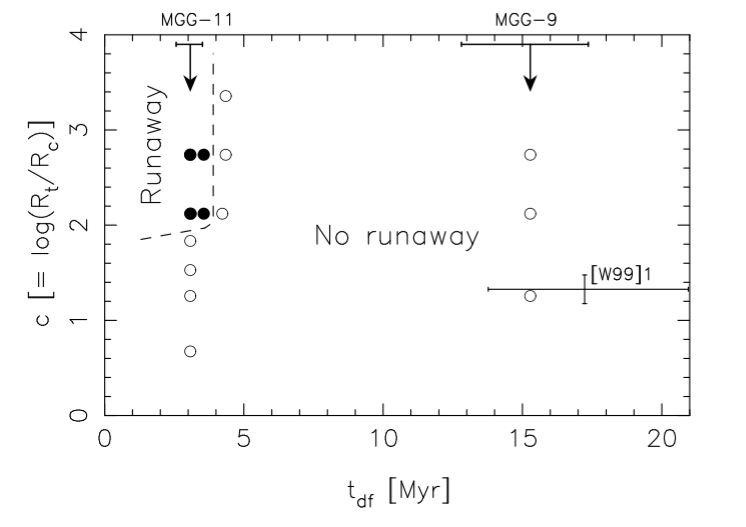
\includegraphics[width=\textwidth]{SPZRunaways}
\caption{This figure, reproduced from \citet{2004SPZ}, shows the range of clusters from their study that produce runaway stars.  Both the concentration and dynamical time are important.  In their study, clusters with lower concentration still had stars with some collisions but were limited to a few hundred solar masses.}
\label{fig:spzrunaway}
\end{figure}

\begin{table}
\begin{center}
\resizebox{0.8\columnwidth}{!}{%
    \begin{tabular}{l l l l l l l }
    \hline \hline \\
    Run & $c_{\mathrm{adj}}$ & $M_{\mathrm{cluster},0}$ & $R_{\mathrm{half, adj}}$ & $t_{\mathrm{df, adj}}$ & $t_{\mathrm{end}}$ & $M_{\mathrm{central, end}}$ \\
    (units) & - & $\msun$ & $\pc$ & $\Myr$ & $\Myr$ & $\Msun$ \\
    \hline
\sc{run64k-w2-m200-r1.5-2} & 1.81 & 2.0e+05 & 0.75 & 1.54 & 0.01 & 268.5 \\
\sc{run64k-w3-m600-r1.5} & 1.94 & 6.0e+05 & 0.75 & 2.22 & 0.01 & 829.9 \\
\sc{run64k-w2-m200-r1.5-3} & 1.78 & 2.0e+05 & 0.75 & 1.54 & 0.04 & 703.2 \\
\sc{run64k-w3-m600-r2.9} & 2.85 & 6.0e+05 & 1.45 & 5.98 & 0.05 & 183.0 \\
\sc{run64k-w3-m2000-r2.9} & 1.94 & 2.0e+06 & 1.45 & 9.20 & 0.06 & 1021.0 \\
\sc{run64k-w2.5-m200-r1.5} & 1.37 & 2.0e+05 & 0.75 & 1.54 & 0.11 & 916.6 \\
\sc{run64k-w1.5-m200-r1.5} & 2.08 & 2.0e+05 & 0.75 & 1.54 & 0.15 & 2598.7 \\
\sc{run64k-w2-m200-r1.5} & 2.04 & 2.0e+05 & 0.75 & 1.54 & 0.32 & 2770.8 \\
\sc{run64k-w3-m200-r1.5} & 1.92 & 2.0e+05 & 0.75 & 1.54 & 0.38 & 429.7 \\
\sc{run64k-w2.5-m600-r2.9} & 1.79 & 6.0e+05 & 1.45 & 5.98 & 0.51 & 163.8 \\
\sc{run64k-w2-m600-r2.9} & 2.37 & 6.0e+05 & 1.45 & 5.98 & 0.79 & 814.7 \\
\sc{run64k-w1.5-m200-r2.9} & 1.65 & 2.0e+05 & 1.45 & 4.15 & 0.82 & 1002.1 \\
\sc{run64k-w2.5-m200-r2.9} & 1.87 & 2.0e+05 & 1.45 & 4.15 & 0.96 & 151.5 \\
\sc{run64k-w2-m2000-r5.8} & 2.46 & 2.0e+06 & 2.9 & 26.03 & 1.14 & 2370.8 \\
\sc{run64k-w1-m200-r2.9} & 2.31 & 2.0e+05 & 1.45 & 4.15 & 1.20 & 1082.9 \\
\sc{run64k-w2-m200-r2.9-3} & 1.60 & 2.0e+05 & 1.45 & 4.15 & 1.26 & 1398.2 \\
\sc{run64k-w2-m200-r2.9-2} & 1.70 & 2.0e+05 & 1.45 & 4.15 & 2.96 & 308.0 \\
\sc{run64k-w2.5-m200-r5.8} & 1.80 & 2.0e+05 & 2.9 & 11.75 & 3.00 & 121.1 \\
\sc{run64k-w1-m200-r5.8} & 2.09 & 2.0e+05 & 2.9 & 11.75 & 3.92 & 844.5 \\
\sc{run64k-w2.5-m600-r5.8} & 2.05 & 6.0e+05 & 2.9 & 16.90 & 4.27 & 315.8 \\
\sc{run64k-w1.5-m600-r5.8} & 1.87 & 6.0e+05 & 2.9 & 16.90 & 4.35 & 1320.9 \\
\sc{run64k-w2-m600-r5.8} & 1.98 & 6.0e+05 & 2.9 & 16.90 & 5.48 & 3204.3 \\
\sc{run64k-w3-m200-r2.9} & 1.71 & 2.0e+05 & 1.45 & 4.15 & 5.98 & 941.0 \\
\sc{run64k-w1.5-m200-r5.8} & -0.18 & 2.0e+05 & 2.9 & 11.75 & 8.68 &  12.8 \\    
        \end{tabular}%
        }
    \caption{Table of each full run (64k bodies), where $c$ is the concentration,  $M_{\mathrm{cluster},0}$ is the initial cluster total mass,  $R_{\mathrm{half}}$ is the initial half-mass radius,  $t_{\mathrm{df}}$ is the dynamical friction time, $t_{\mathrm{end}}$ is the simulation end time, and  $M_{\mathrm{central, end}}$ is the ending central mass size. \textsc{run64k-w1.5-m200-r5.8} shows a negative value for $c_\mathrm{adj}$ because our correction did not account for an increase in the edge radius.}
    \label{tbl:runs}
\end{center}
\end{table}
\section{Parameter Corrections}
Some aspects of our run parameters surprised us.  Each run began with almost zero kinetic energy, and so rapidly underwent collapse into a more stable configuration.  In order to reach virial equilibrium, the cluster half-mass radius drops by approximately a factor of two.  We also measured the change in the cluster core radius to get the adjusted concentration, given by the following equation:
\begin{equation}
c_{\mathrm{adj}} = c + \log_{10} \frac{r_{\mathrm{core},0}}{r_{\mathrm{core, collapse}}}.
\label{eqn:cadj}
\end{equation}
This led to an increase in concentration of between $1$ and $2$ per run, for most runs. This estimate for the adjusted concentration is likely conservative, because it assumes the edge radius of the cluster does not change.  If the edge radius also increases, the adjusted concentration would be higher. We also adjust $t_{\mathrm{df}}$ by a factor of $1/\sqrt{8}$ to account for the decrease in half-mass radius. Both Table~\ref{tbl:runs} and the figures in this section use the adjusted values for $c$ and $t_{\mathrm{df}}$. With this adjustment, our parameter space is comparable to both observed clusters and the work of \citet{2004SPZ}.

\section{Determining Runaway Candidates}
We performed simulations of 24 clusters sampling the parameter space of concentration, cluster mass, and core radius, as detailed in Table~\ref{table:runs}. We targeted an end time of $3 \Myr$ for each cluster to reach the end of life for the most massive stars in the cluster. Because of the computational difficulty of simulating collisional clusters with many bodies, not all of the runs made it to completion. Figure~\ref{fig:JobProgress} shows the suite of runs and their end times, as well as the size of their final central masses. As many simulations only make it to $\sim 0.1 - 0.5 \Myr$ before they become too difficult to simulate, comparing the results of different clusters requires normalizing for time. However, we can still make a guess as to whether a runaway should occur, even if projecting the mass of the star to $3 \Myr$ is difficult. To do this, we suppose that the early stages of massive star growth can be modeled as an exponential such that
\begin{equation}
    M_{\mathrm{max}}(t) = M_{0} e^{(Kt)}.
    \label{eqn:expcluster}
\end{equation}
We can see that $1/K$ is the time required for one e-folding, and solve for $K$ at the end of a given run by isolating it from equation~\ref{eqn:expcluster} as follows:
\begin{equation}
K = \frac{\ln M_{\mathrm{max}}(t_{\mathrm{end}}) - \ln M_{0}}{t_{\mathrm{end}}}
\end{equation}
We can then use $K$ to make an estimate for the central mass size as a fraction of the cluster at $t = 3 \Myr$.  If the projected final mass fraction is large, we suggest the cluster is a candidate to have a runaway central mass. Figure~\ref{fig:Kplot} shows each run plotted with its projected final mass fraction.

Perhaps more informatively, we can project when the central mass would reach $10^4 \Msun$, which is still only between $1-5\%$ of the overall cluster mass, and doesn't require the exponential growth to continue far outside of a similar cluster than those we simulated.  Using this estimate, we see that our runs which already have runaway stars project central masses of $10^4 \Msun$ between about $0.5$ and $10 \Myr$. This result is quite encouraging and suggests that more efforts should be made to simulate clusters out to these times.

\section{Clusters with Potential Runaway Stars}
Some of our runs contain central masses that reach $> 1\%$ of the total cluster mass on timescales of only $\sim 0.1 \Myr$.  Figure~\ref{fig:MaxMass2-200-1.5} shows the growth of one such case. The central mass reaches over $2700 \Msun$ by $t = 0.3 \Myr$, or about $1.3 \%$ of the cluster mass in $10\%$ of the limiting time. The growth rate starts off superexponential as the stars initially come into contact, and the massive star continues to attract collisions throughout the run.  Compared to the results of \citet{2004SPZ}, our collisional clusters tend to have more massive runaways more quickly, as even their most massive runaway stars reach $2500 \msun$ at about $t = 3 \Myr$, as shown in Figure~\ref{fig:CompareGrowth}.
\begin{figure}%
    \centering
     \subfloat[Growth of the collision runaway star vs. time reproduced from \citet{2004SPZ}.]{{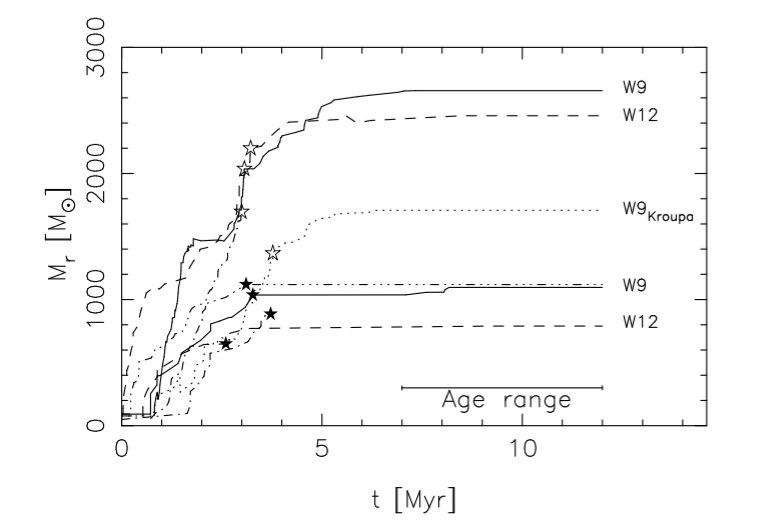
\includegraphics[width = 0.8\textwidth]{SPZGrowth}}}%
    \qquad   
    \subfloat[Growth of the collision runaway star vs. time from our experiments.]{{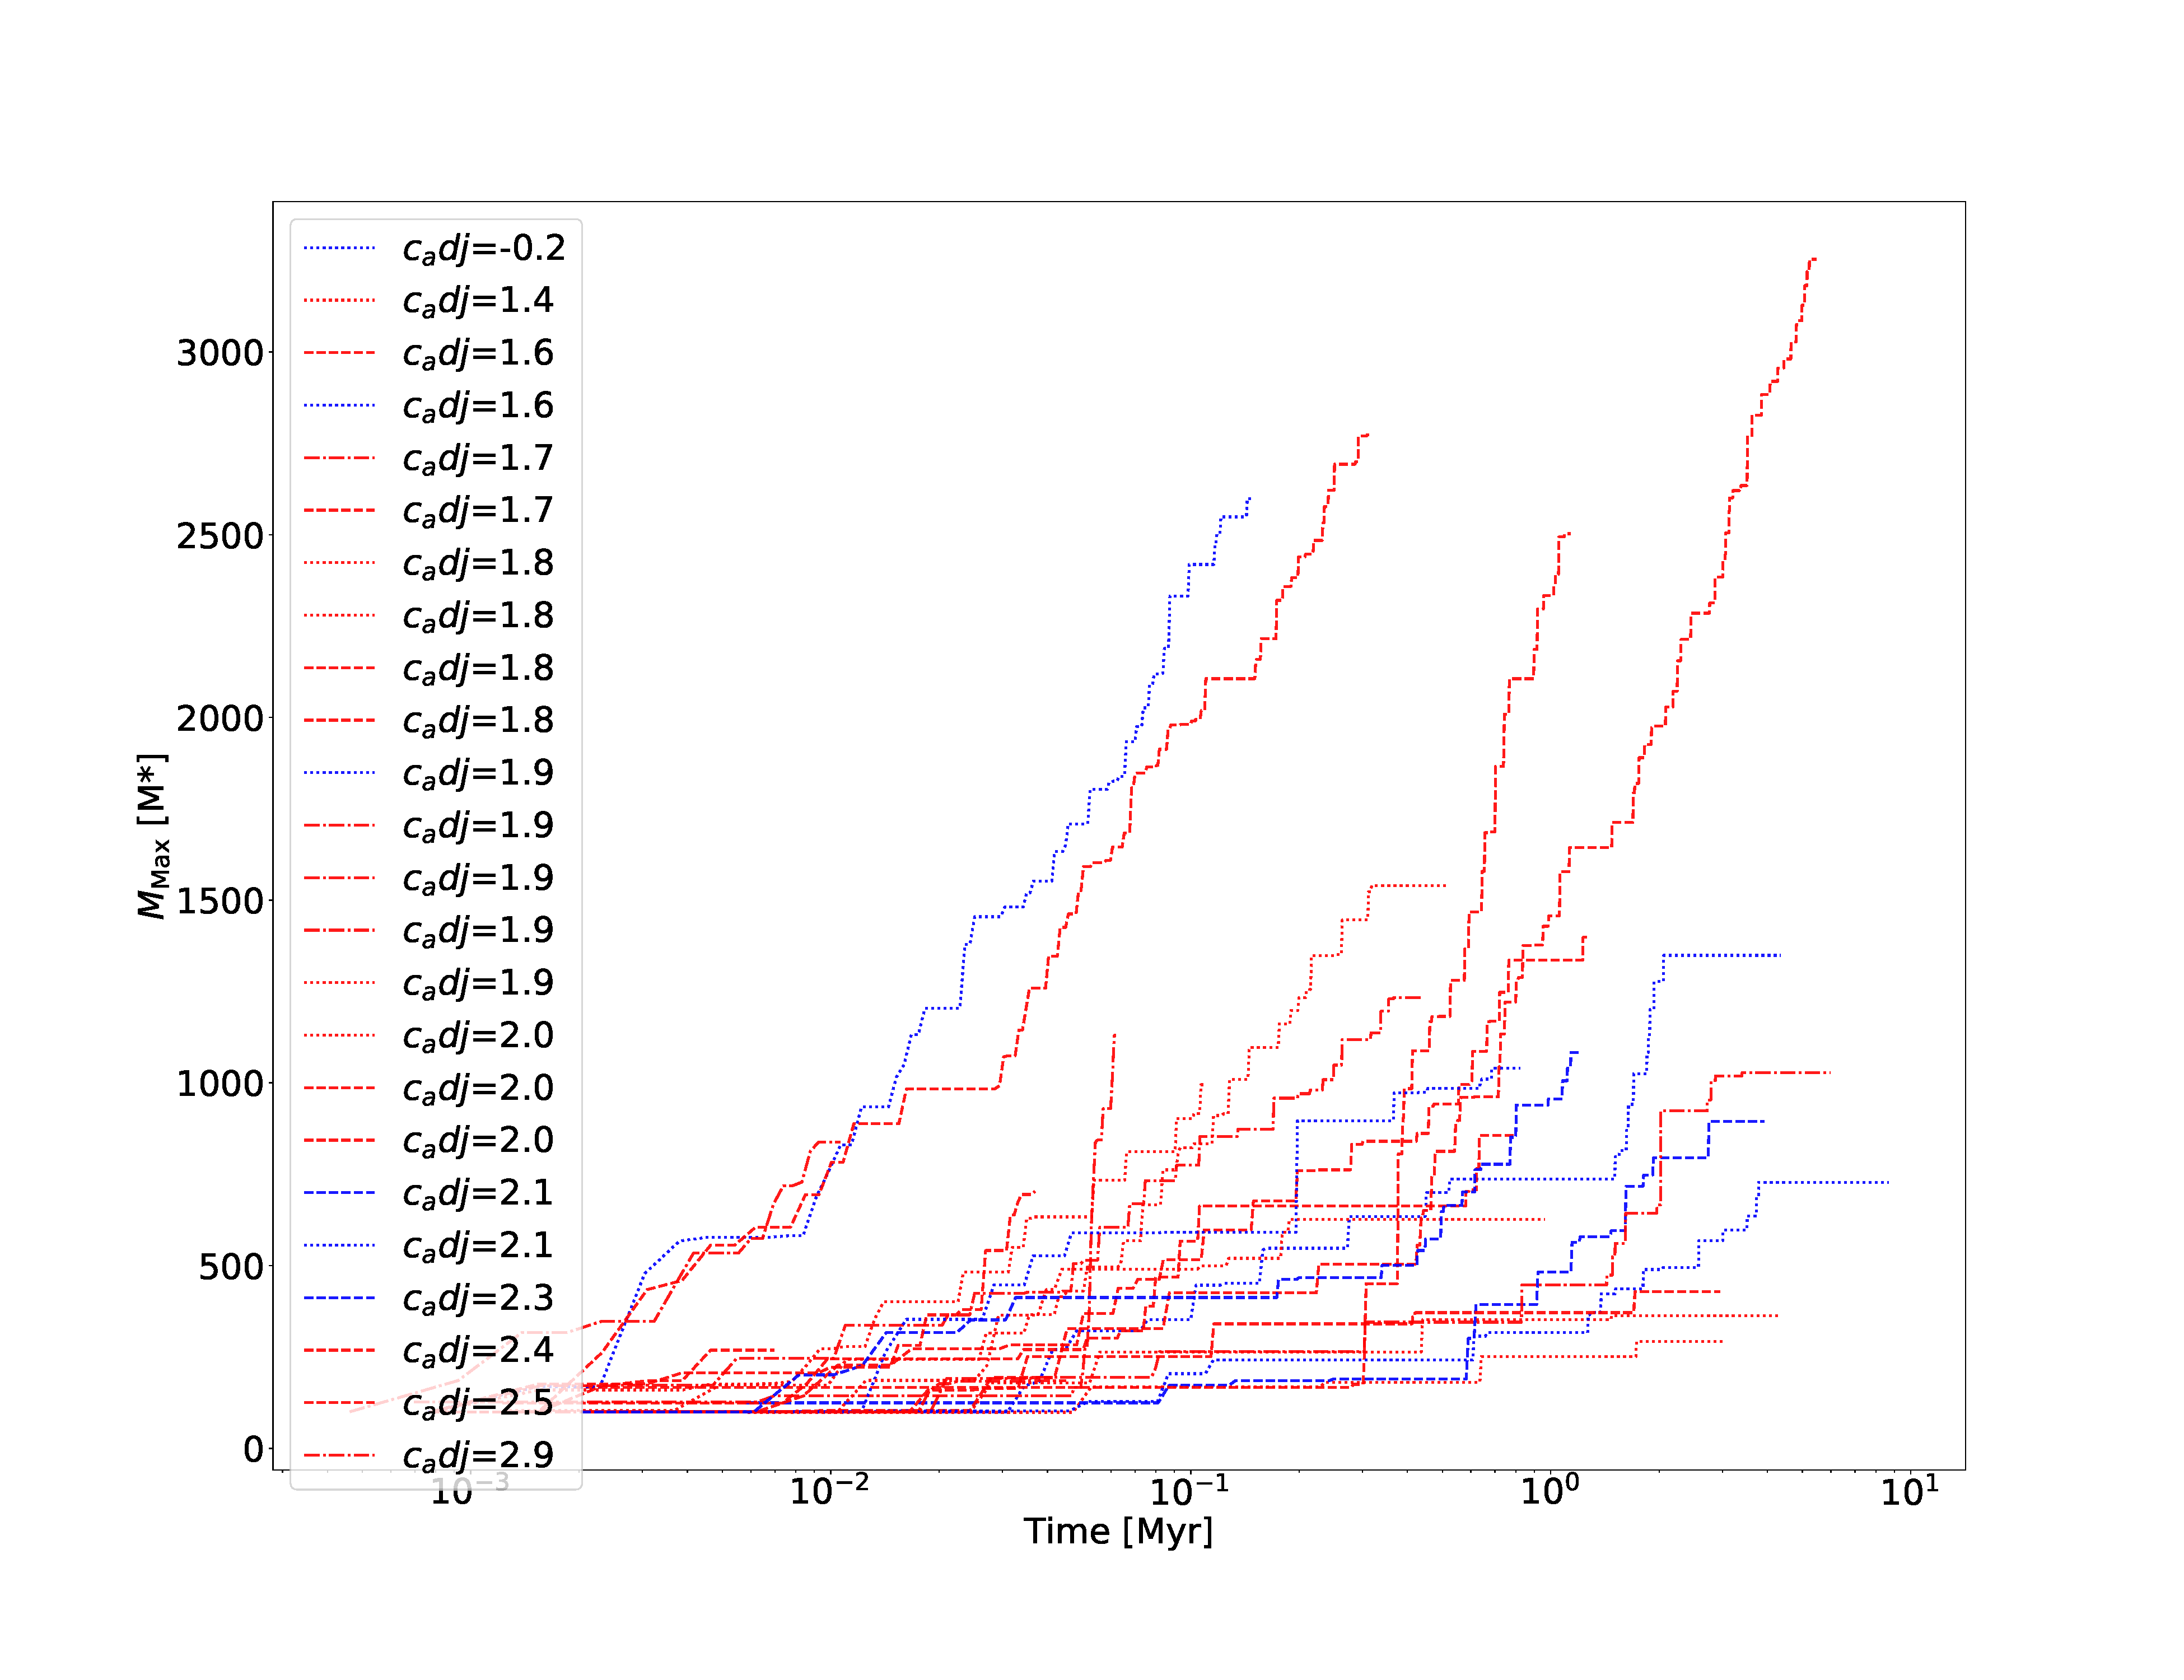
\includegraphics[width = 0.8\textwidth]{allgrowth}}}%
    \caption{Here we compare the growth of collision runaways from }
    \label{fig:CompareGrowth}
\end{figure}
Although our simulations do not run for as long, they do achieve comparable central masses in a fraction of the time.  Assessing the differences, both our $200 \times 10^5 \msun $ and $600 \times 10^5 \msun$ experiments are comparable to the $300 \times 10^5 \msun$ used in their simulations. Our $2 \times 10^6 \msun$ clusters are larger than the ones in their simulations.  The adjusted concentrations and dynamical friction times are in similar ranges, so it's possible that the main change is in the underlying distribution after the initial collapse to virial stability.  It's also possible that we've more significantly undercounted the true concentration. If the edge radius in fact increases by a factor of 5-10, this could add an additional 0.7-1 to the adjusted concentration.  On the high end of the scale, this would take our clusters beyond the range probed by \citet{2004SPZ}.

Figure~\ref{fig:Kplot} shows that while in general higher concentration and lower dynamical friction time corresponds to runaway mass, the total cluster mass has an effect as well. We see that \textsc{run64k-w2-m2000-r5.8}, which has the greatest $t_{\mathrm{df}}$ at  has a central mass of $2400 \Msun$ at $t = 1 \Myr$, so there is some potential to reach a mass of $\sim 10^4 \Msun$ by $3-4 \Myr$.  This run does use a shallow concentration parameter of $c \approx 0.5$, but all the runs with nearby values of $t_{\mathrm{df}}$ and smaller cluster masses do not exhibit runaways.  The remaining runaways appear at only substantially smaller $t_{\mathrm{df}}$ values of $< 10 \Myr$.

Another factor that may influence the comparison between our work and that of \citet{2004SPZ} is the total number of bodies. They have a similar cluster mass on the order of $10^{5} \Msun$, but extend the lower bound of their initial mass function to $0.08 \Msun$.  Most of their simulations are performed with 128k stars, with some performed with 585k stars.  It's possible that a greater number density of stars could lead to more collisions, even if most of the stars are less massive, because the impact parameter of the high-mass stars would remain the same. If the number density is higher overall, this would allow for more chances for high-mass stars to capture additional mass.

We also suspect there is some sensitivity to the instantiation of the initial distribution, even for clusters with the same parameters. Near boundaries in the parameter space, there is no guarantee of forming the first few collisions to kick off the process of massive star formation. Figure~\ref{fig:SameParamsMassTime}, shows that for our three runs with the same parameters but differential initial masses, positions, and velocities: \textsc{run64k-w2-m200-r2.9, run64k-w2-m200-r2.9-2} and \textsc{run64k-w2-m200-r2.9-3}, two formed massive stars above $10^3 \Msun$ and one did not.

In general, collision counterparts were more massive stars above $\sim 30 \Msun$. The first two to three tended to be stars above $50 \Msun$, which appears to kickstart the collision process in general. In their study, \citet{2004SPZ} found the same trend, and it appears to persist throughout the life of the massive star. In our clusters with mass $2 \times 10^6$, which have stars with an initial maximum mass of $120 \Msun$, we see most collision counterparts are above $100 \Msun$.  If mass segregation occurs early in the life of the cluster, we might expect to see only massive stars near the central mass, which could also explain why most collision counterparts are the most massive stars initially.
\begin{figure}
\centering
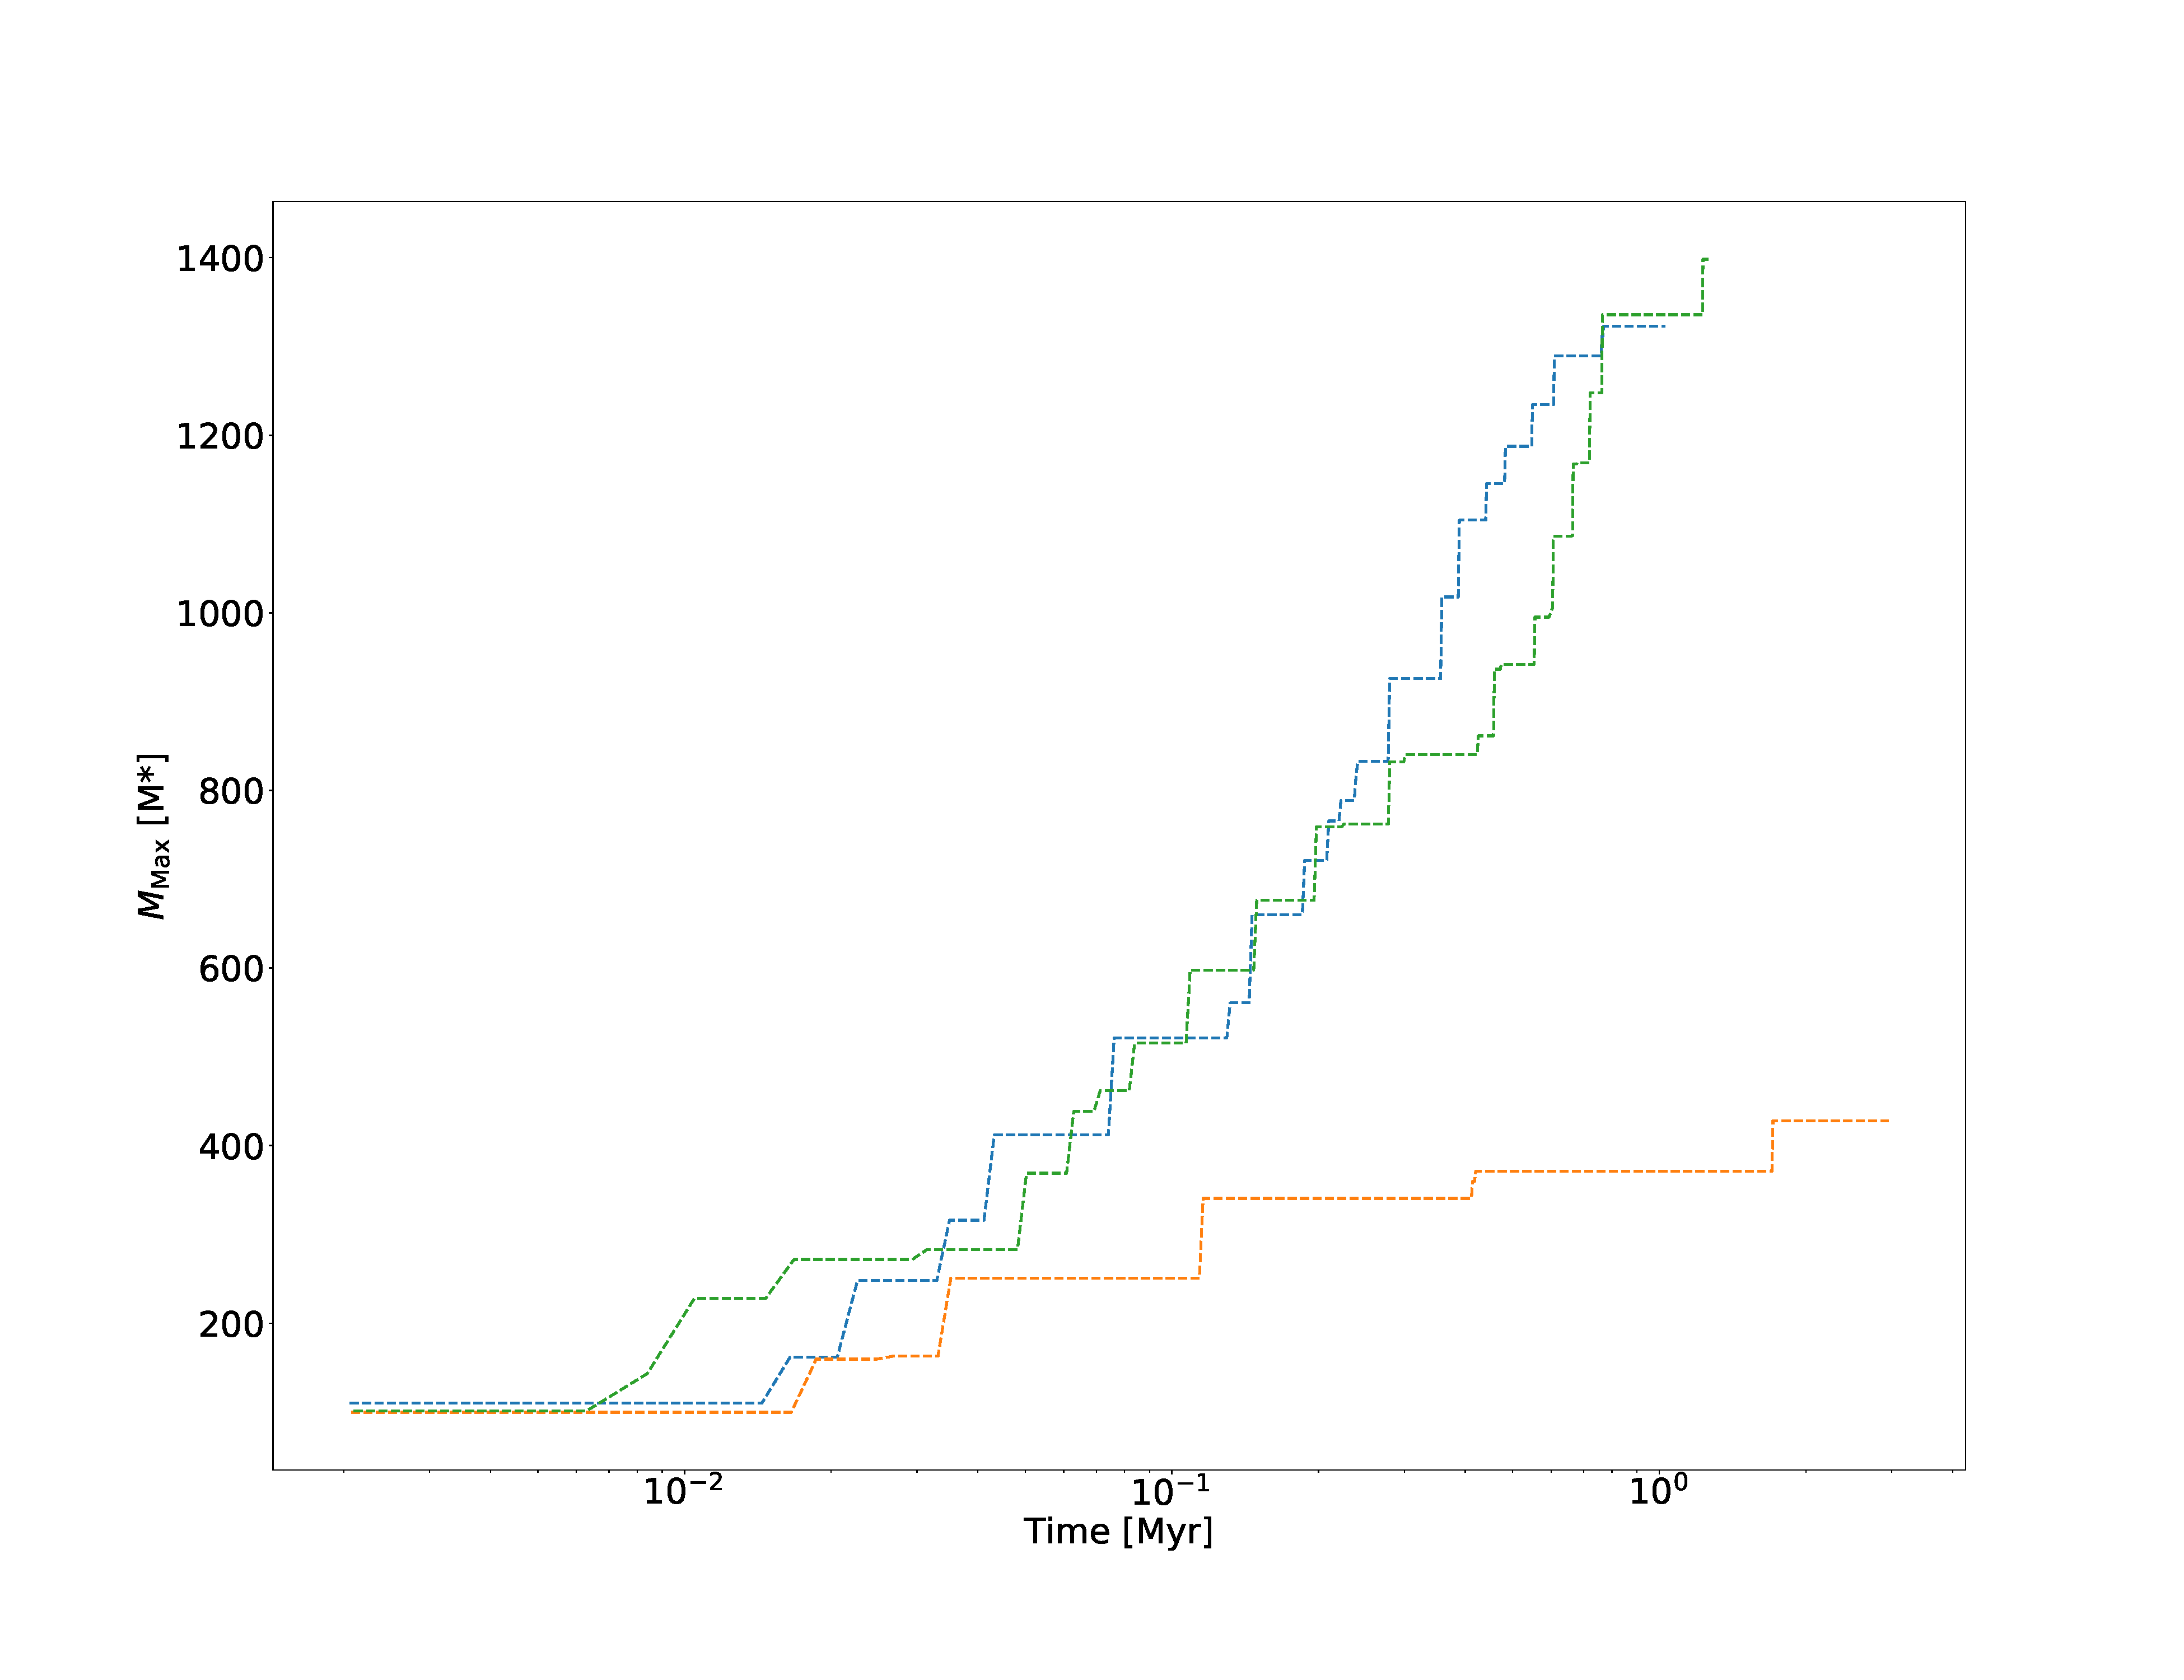
\includegraphics[width=\textwidth]{masstimesame}
\caption{Two runs demonstrate growth at comparable rates to > $10^3 \Msun$, but in one run no real runaway occurs.}
\label{fig:SameParamsMassTime}
\end{figure}

\begin{figure}
\centering
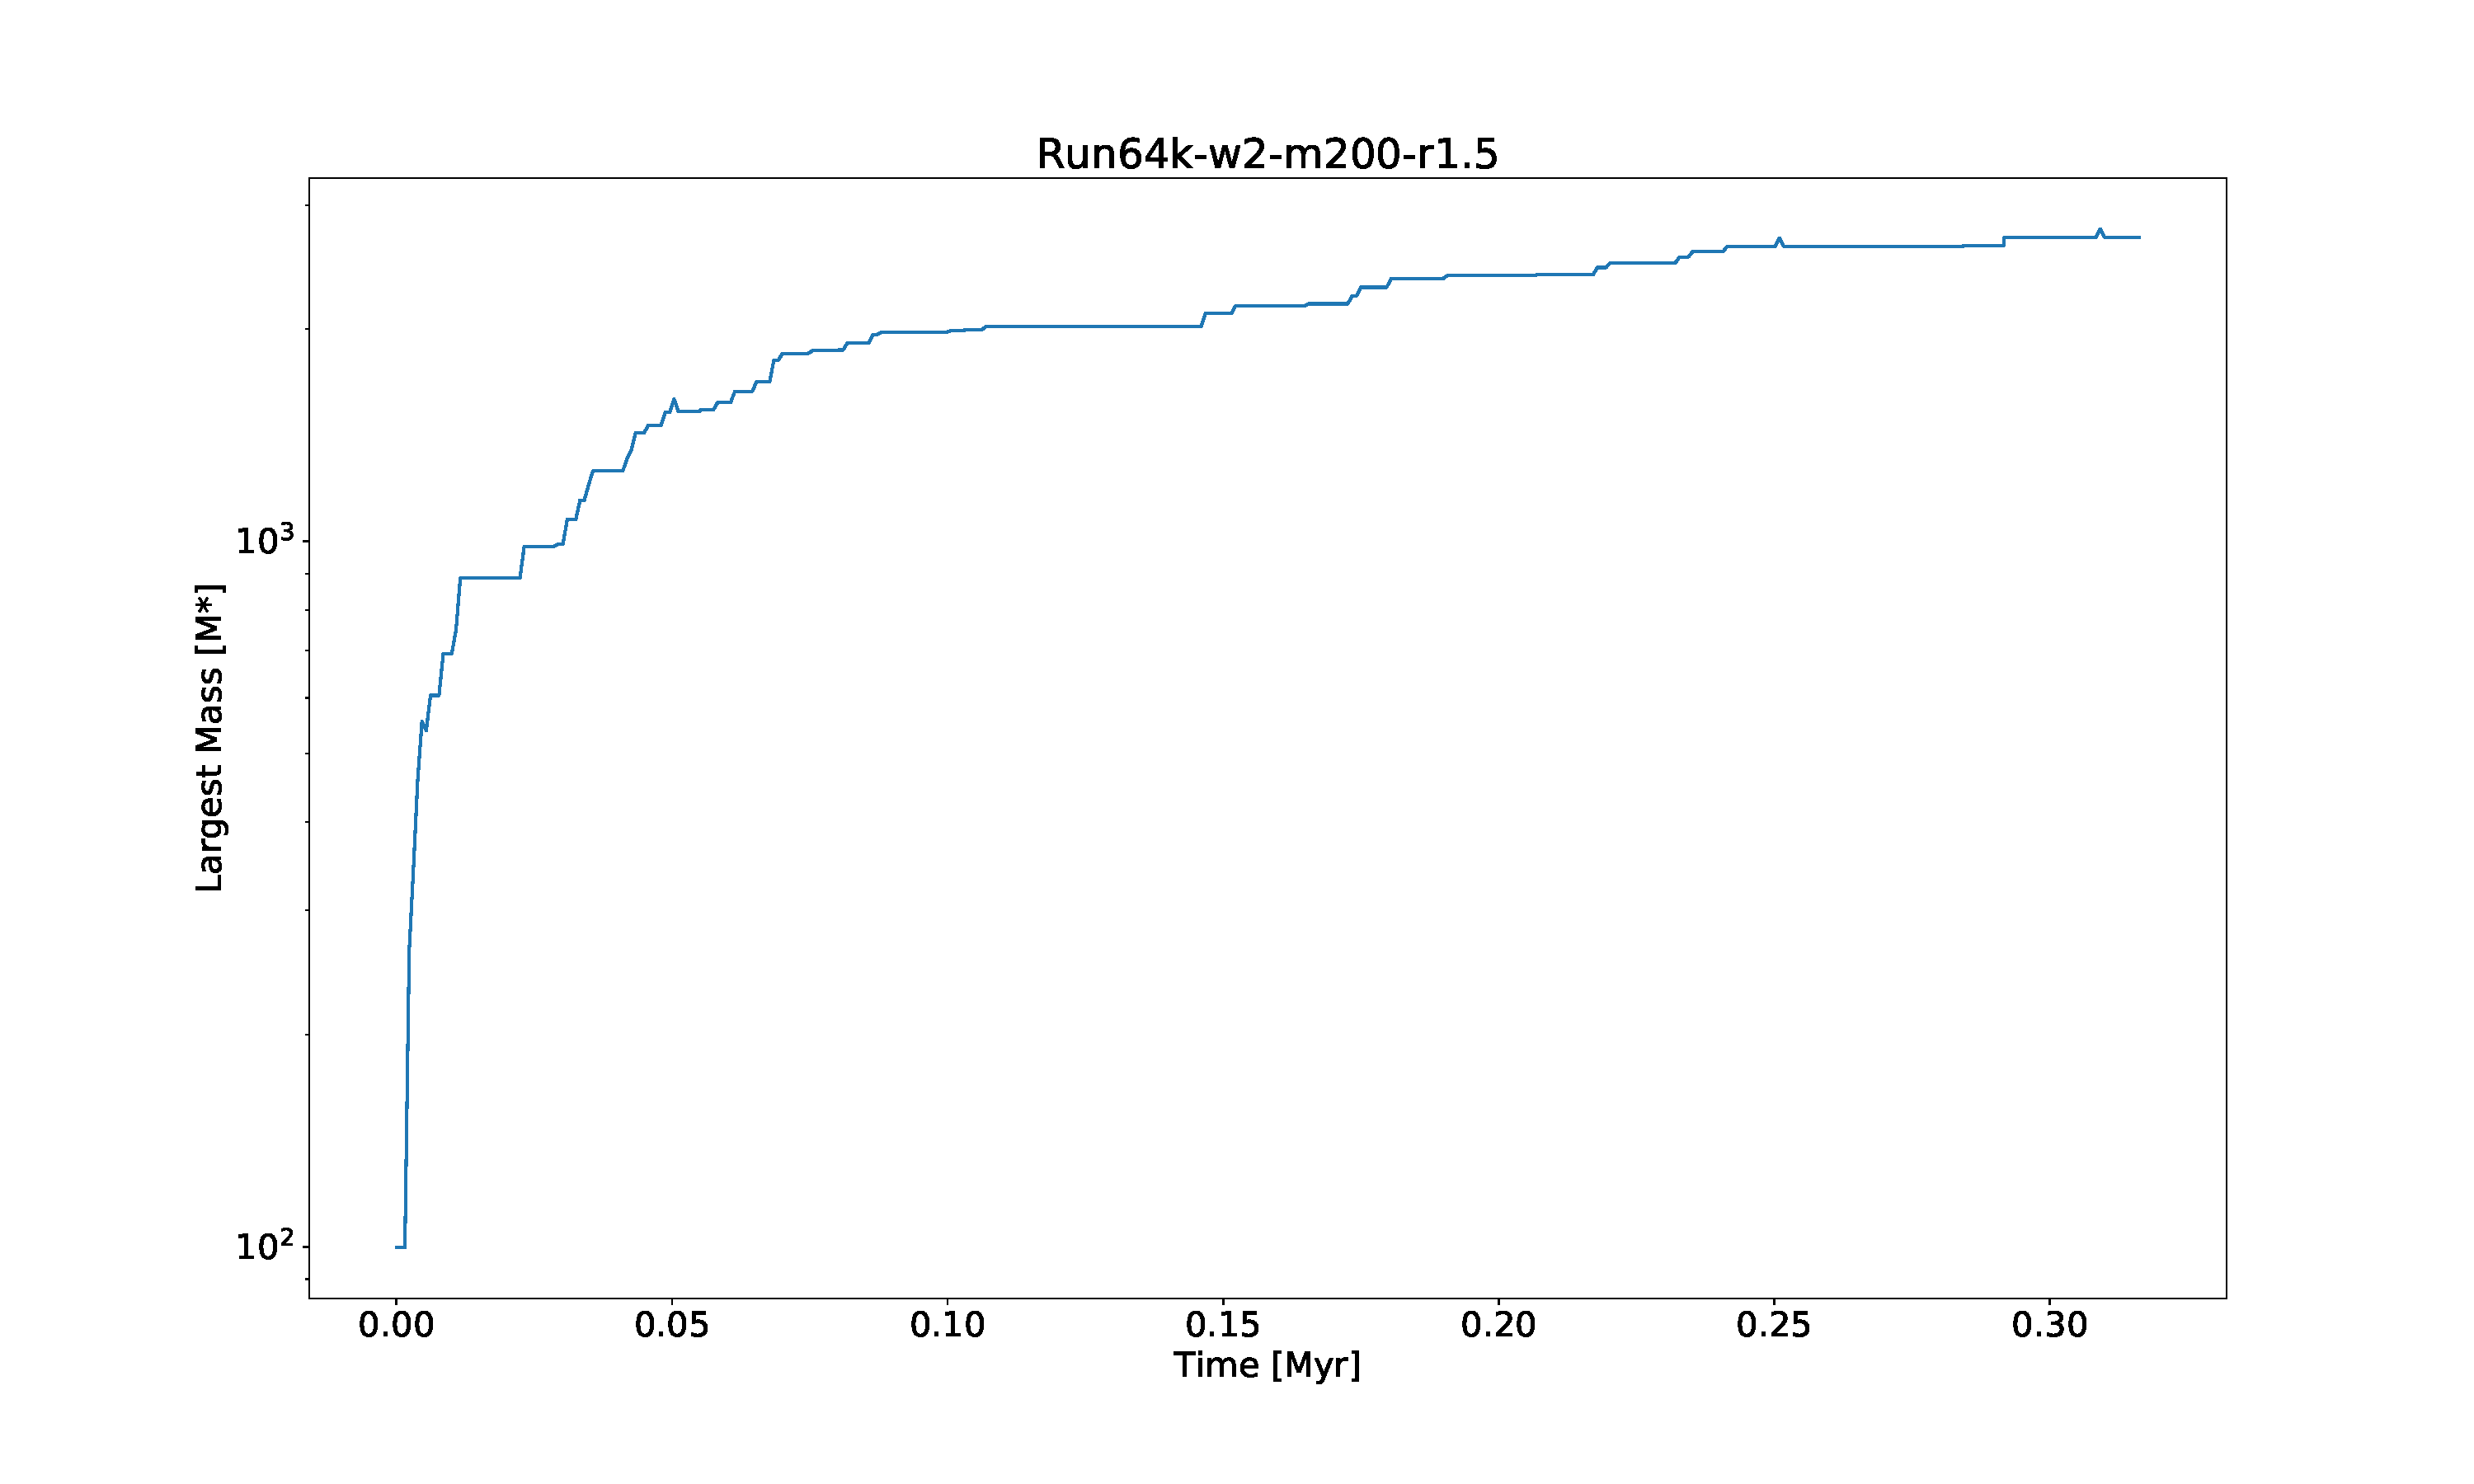
\includegraphics[width=\textwidth]{MaxMassTime2-200-15}
\caption{This plot charts the growth of the runaway star from $100 \Msun$ to approximately $2700 \Msun$ in a cluster with a half mass radius of 0.75 pc, a concentration parameter of 0.4, and a total mass of $200 \times 10^5 \Msun$. Bumps in the curve are the result of multiples where the smaller member escapes instead of merging. Collisions continue until the end of the simulation.}
\label{fig:MaxMass2-200-1.5}
\end{figure}

\begin{figure}
\centering
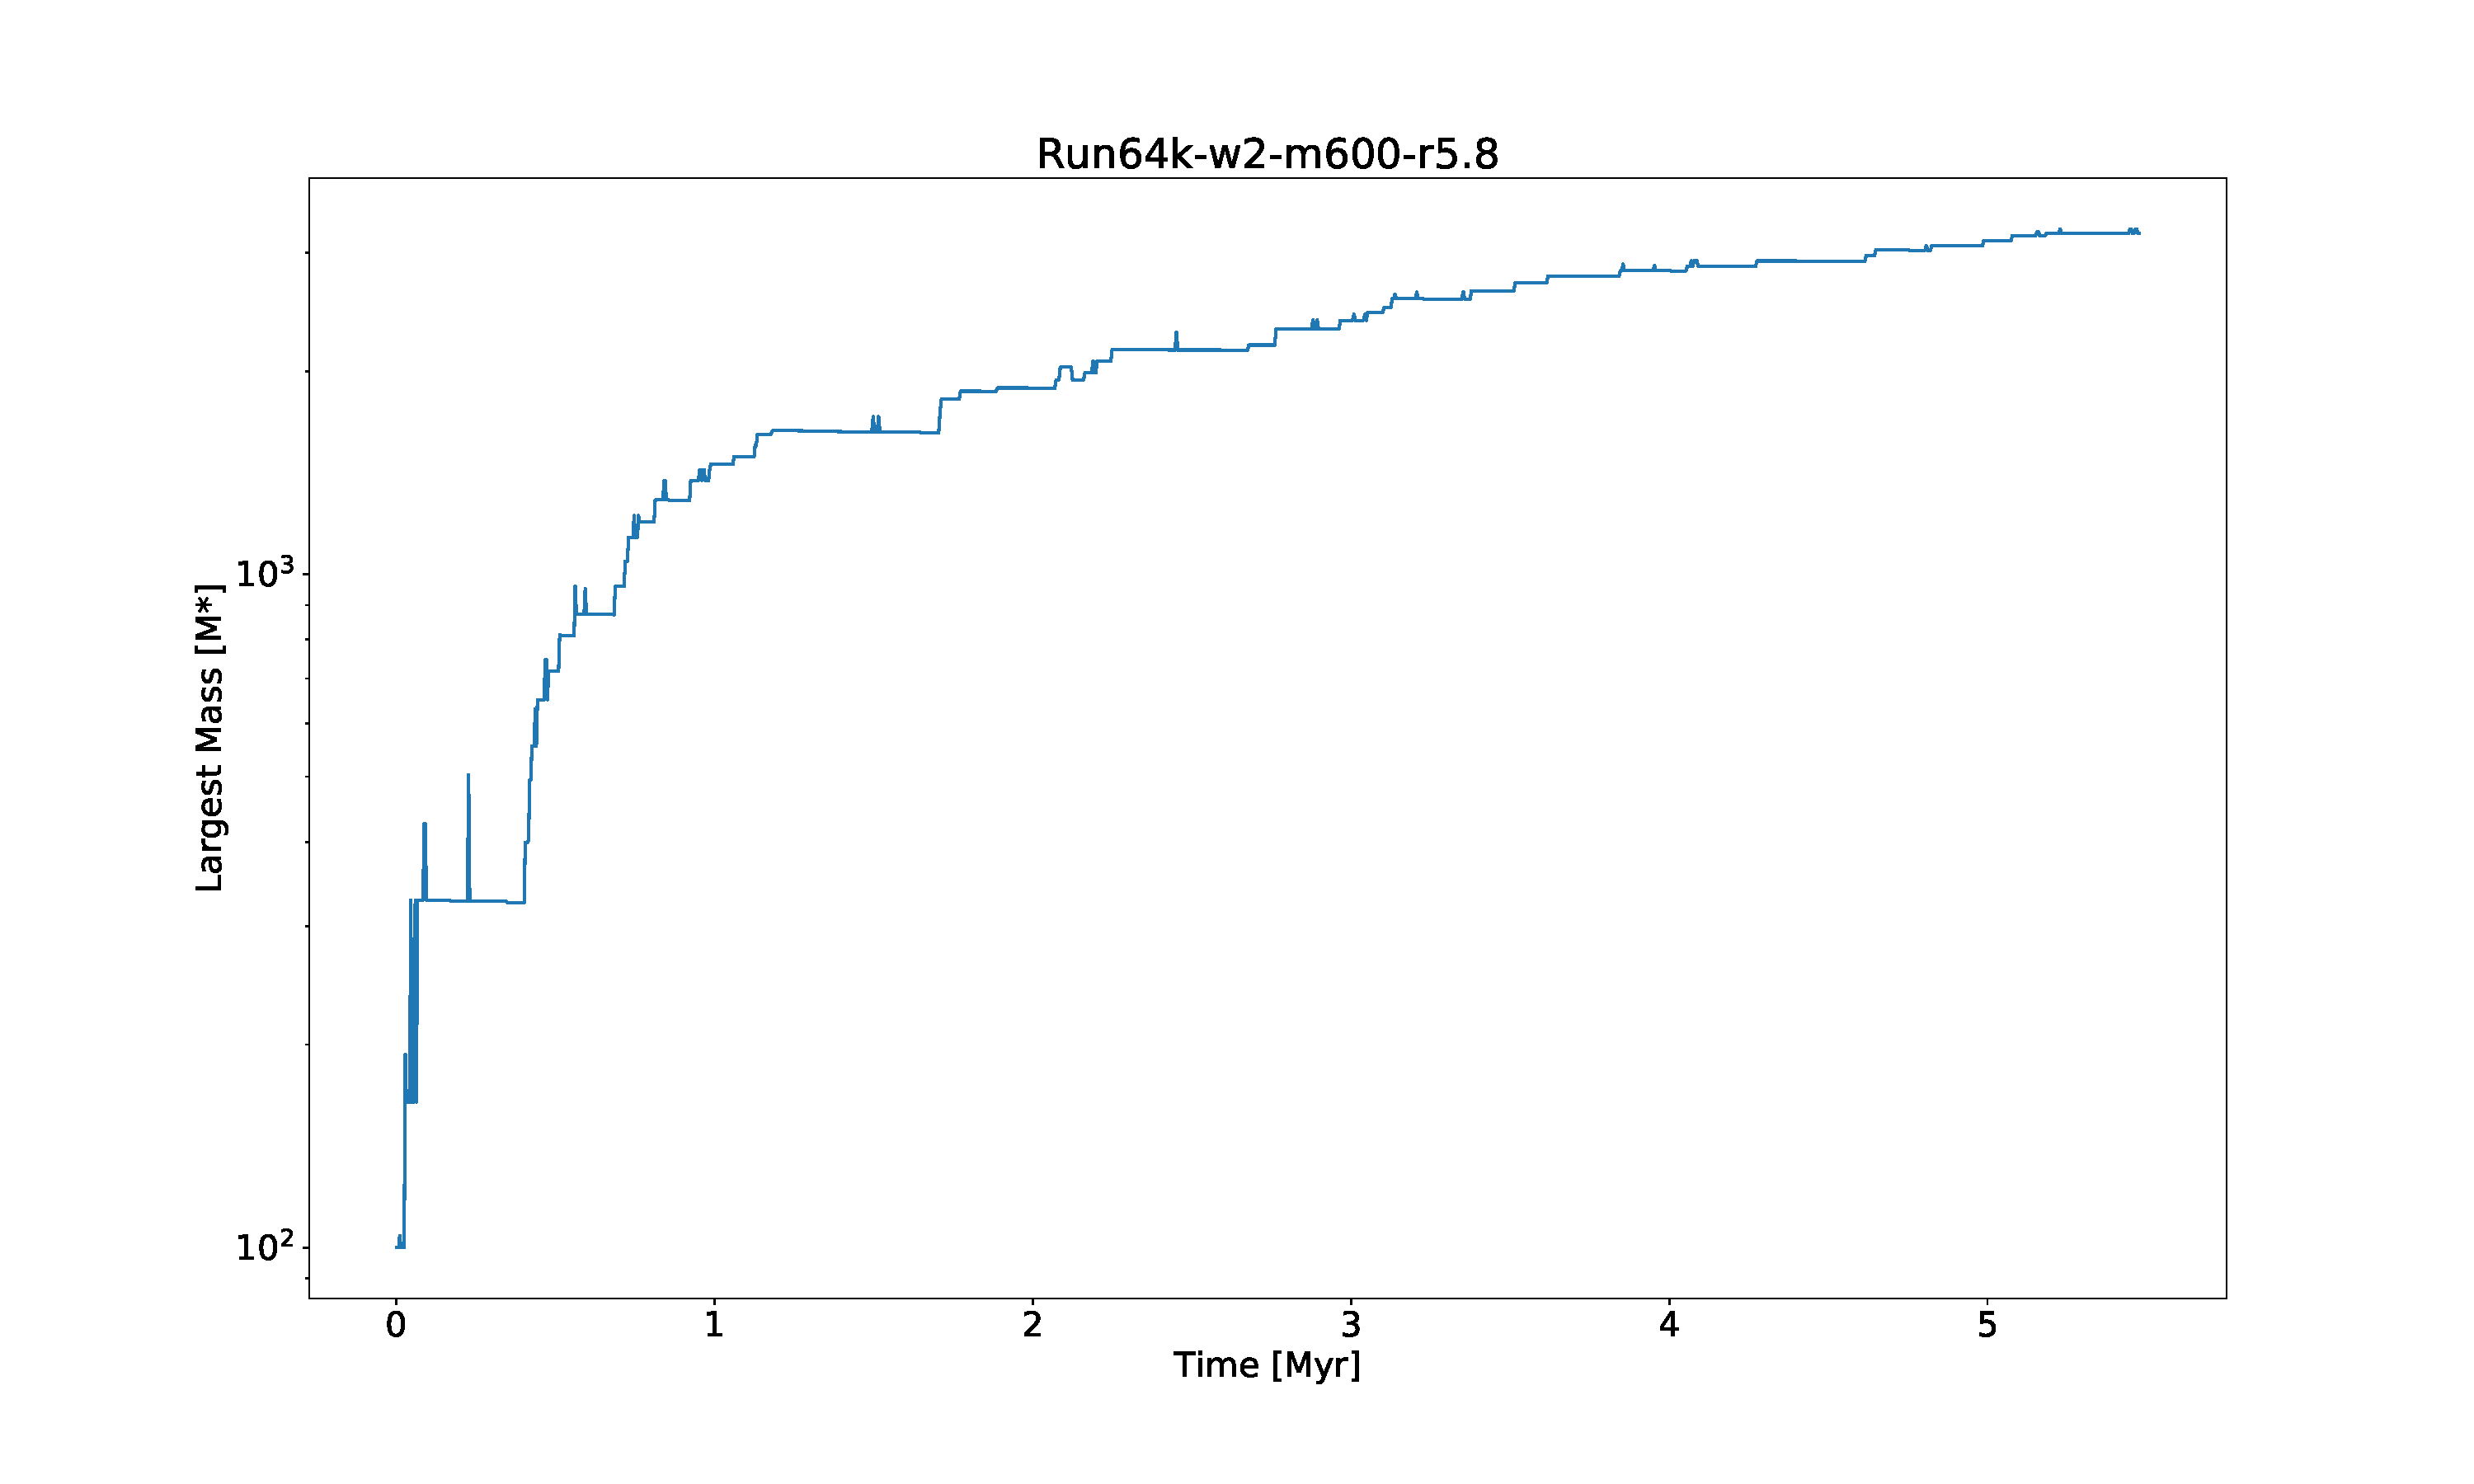
\includegraphics[width=\textwidth]{MaxMassTime-2-600-58}
\caption{The central star in this plot grows more slowly and at rates commensurate with those in \citet{2004SPZ}.  However, it appears that the star is still colliding at the end of the run instead of reaching a steady state. This cluster has a $t_{\mathrm{df}}$ of $\sim 15 \Myr$.}
\label{fig:MaxMass2-600-5.8}
\end{figure}

All clusters had some mass loss, primarily because of escapers. The total number of particles in the system decreases with escapers and mergers, and the decrease in particle number appears to be commensurate with mass loss, suggesting that there's not a big difference between the masses of ejected and retained particles. To normalize for different initial masses and run lengths, we consider the cluster ``evaporation time,'' defined as 
\begin{equation}
    t_{\mathrm{evap}} = \frac{M_{0}}{\left(\frac{\Delta M}{\Delta t}\right)}.
\end{equation}
Figure~\ref{fig:EvapKplot} shows the evaporation time plotted against the $e$-folding time $1/K$. Clusters with higher values of $K$ tend to have shorter evaporation times, but overall most are around $10 \Myr$.  As long as the evaporation time is longer than the lifetime of the most massive stars in the cluster, we expect the latter will provide the main constraint on whether a SMS may form.
\begin{figure}
\centering
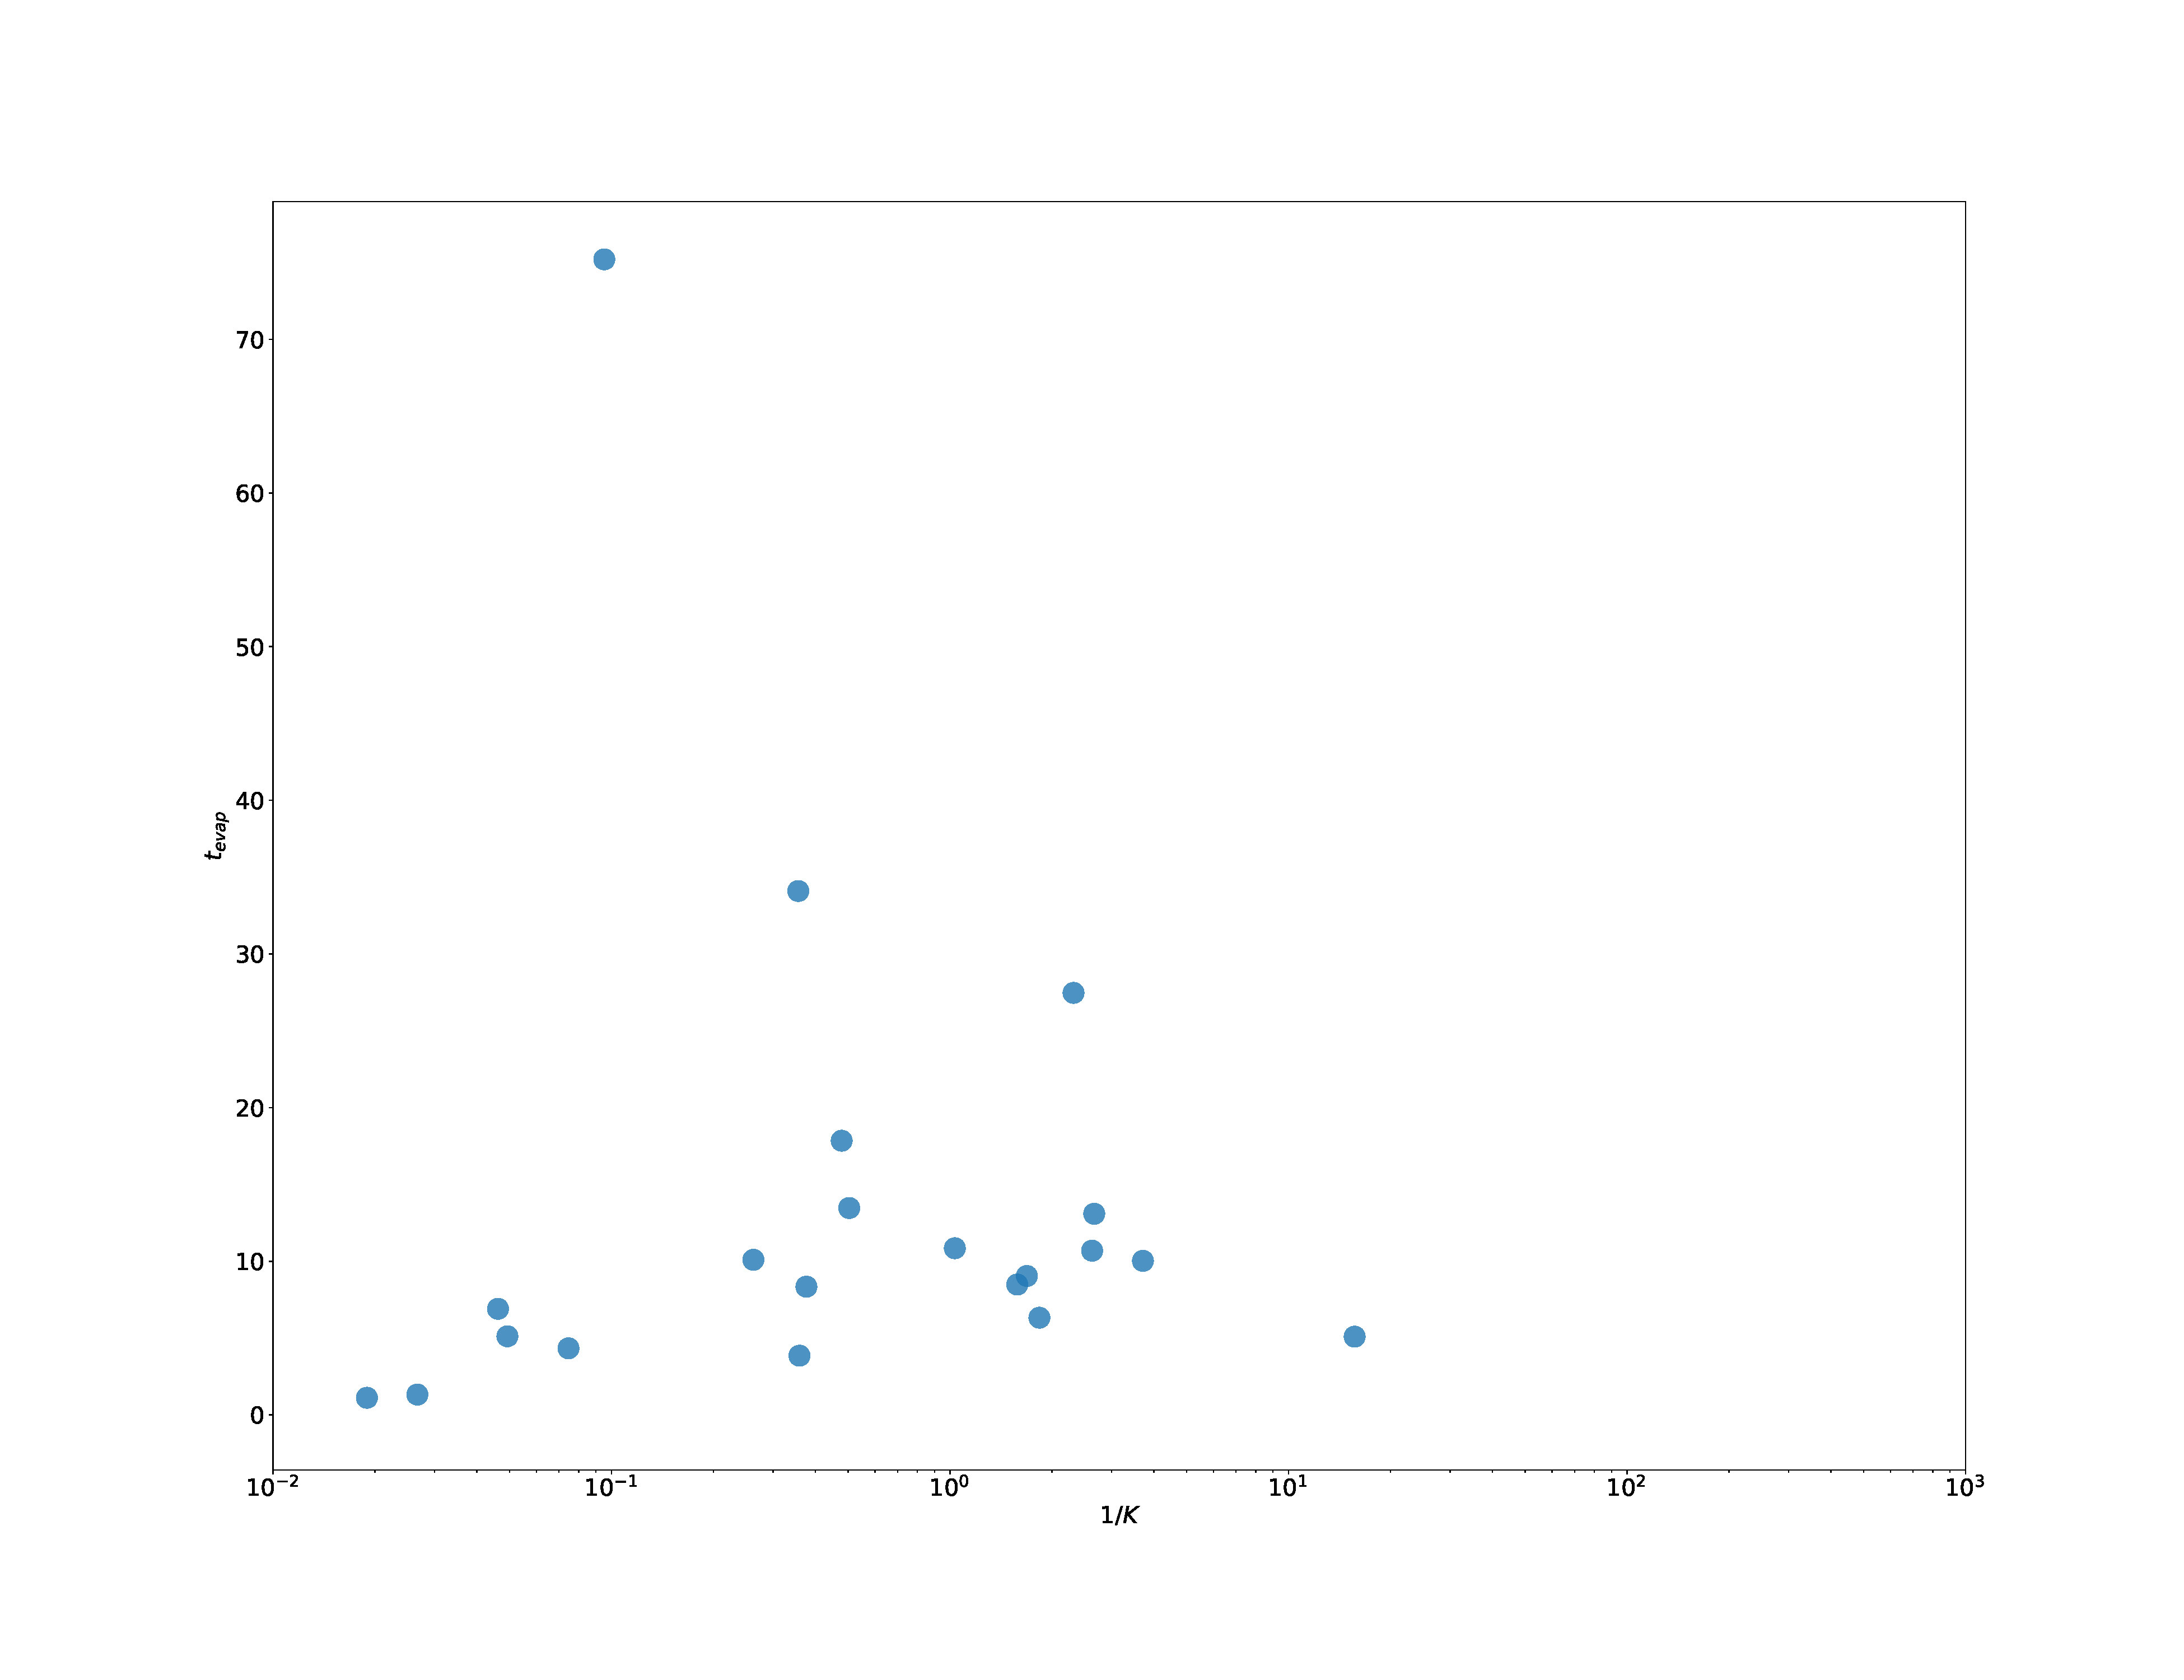
\includegraphics[width=\textwidth]{kevap}
\caption{$1/K$ vs. $t_{\mathrm{evap}}$ for all clusters.}
\label{fig:EvapKplot}
\end{figure}

\section{Clusters without Runaway Stars}
Some of our clusters ended with maximum mass stars of only a few hundred solar masses. Such stars were generally formed by collisions of only a couple of the most massive stars in the cluster, but then appeared to run out of steam. Most of these clusters had higher dynamical friction times.  Consequently, we would expect to see fewer massive stars near the core, and it appears that the presence of the most massive stars is required to add enough mass to the runaway. 

\chapter{Conclusions} \label{ch:Conclusions}
In this work we examined one possible pathway for \ac{SMBH} formation through ambituous simulations of highly collisional globular clusters. Though we broadly probe a range of parameters informed by observation, we recognize a challenge in observationally constraining the boundaries of the parameter space, as clusters most prone to forming SMSes via runaway would have done so already.

Although we faced challenges in simulation execution and have not yet probed the full parameter space of plausible clusters, we remain cautiously optimistic that repeated collisions can lead to runaway star growth.  Qualitatively, our results generally agree with previous experiments. Quantitatively, we see the potential for runaway star formation up to $10^4 \Msun$ well before the cluster should experience disruption from supernovae or tidal evaporation. As numerical methods, simulation software, and computing capacity improve, it should be possible to simulate clusters with $\sim 10^6$ stars for several million years which will provide more conclusive results.

One significant question mark left in our experiments is the rapid collapse to virial equilibrium from the initial position-only King profile.  Understanding whether the ensuing profile is really a plausible initial condition is likely to be important for assessing the physical viability of our results.  

Future investigators may also want to consider additional parameters. Variations in the initial mass function and maximum mass of the earliest stars could have implications for both the critical time limit and for the initial collisions that form runaway stars. Simulating clusters with the same bulk properties but different particle counts might also prove informative. Adding a galactic tidal force may also have implications for particle removal at the edges of clusters. Exploring a range of $W_{0}$ from approximately $8 - 15$ ($c$ from $2 - 4$), will offer more exposure to the higher end of the range of observed clusters and somewhat beyond. We also performed our simulation without primordial binaries or primordial mass segregation, both of which would tend to increase the merger rate and chances of runaway.  The behavior of supermassive stars formed by many collisions may also prove a fruitful area of investigation.

In addition to the work described in the rest of this paper, we have also made efforts to ensure our research is repeatable and extendable. We have made available our suite of scripts for configuring and performing experiments and analysis at \url{www.github.com/efrubin/thesis-scripts}, and welcome contributions.


\bibliographystyle{apj}
\bibliography{ref}
\nocite{*}
\acrodef{SMBH}{supermassive black hole}
\acrodef{IMBH}{intermediate-mass black hole}
\end{document}